% ====================================================================
% graphite_ica_ch1_v8-08.tex -- Chapter 1 v8 derivation-restored edition
% Source layout/result preservation target: Claude/results/v7-11/v7-11.tex
% Derivation source: Claude/docs/graphite_ica_ch1_Opus_v5.tex
% Code/sign spine: Claude/results/v7-00_spine/Anode_Fit_v11_final.py and v11_flowchart.md
% ====================================================================
\documentclass[11pt,a4paper]{article}
\usepackage[margin=22mm]{geometry}
\usepackage{kotex}
\setmonofont{D2Coding}[Scale=MatchLowercase]
\usepackage{amsmath,amssymb,mathtools,bm}
\usepackage{booktabs,longtable,array}
\usepackage{enumitem}
\usepackage{amsthm}
\usepackage{hyperref}
\usepackage{fancyhdr}
\usepackage{lastpage}
\usepackage{setspace}
\usepackage{tikz}
\usetikzlibrary{positioning,arrows.meta,calc,fit,backgrounds}
\setstretch{1.12}
\setlength{\parskip}{0.45em}\setlength{\parindent}{0pt}\setlength{\headheight}{14pt}
\setlength{\emergencystretch}{2em}
\hypersetup{colorlinks=true, linkcolor=blue, urlcolor=blue, citecolor=blue,
  pdftitle={흑연 음극 dQ/dV 이론: 코드 진행을 따라가는 수식-구동 — Chapter 1 (v8-08)}}
\pagestyle{fancy}\fancyhf{}
\lhead{흑연 음극 $dQ/dV$ 이론 — Ch.1 (v8-08, 유도 복원판)}\rhead{\thepage/\pageref{LastPage}}
\renewcommand{\headrulewidth}{0.4pt}

\newtheorem*{keybox}{핵심}
\newtheorem*{codebox}{코드 대응}
\newtheorem*{signbox}{부호 검산}
\newtheorem*{verifybox}{검산}
\newtheorem*{derivebox}{유도 복원}

\newcommand{\dd}{\mathrm{d}}
\newcommand{\eff}{\mathrm{eff}}
\newcommand{\eq}{\mathrm{eq}}
\newcommand{\app}{\mathrm{app}}
\newcommand{\cell}{\mathrm{cell}}
\newcommand{\bg}{\mathrm{bg}}
\newcommand{\rxn}{\mathrm{rxn}}
\newcommand{\dis}{\mathrm{dis}}
\newcommand{\chg}{\mathrm{chg}}
\newcommand{\hys}{\mathrm{hys}}
\newcommand{\work}{\mathrm{work}}
\newcommand{\rep}{\mathrm{rep}}
\newcommand{\code}[1]{\texttt{#1}}

\renewcommand{\theequation}{1.\arabic{equation}}
\renewcommand{\thesection}{1.\arabic{section}}
\title{\textbf{\LARGE Chapter 1}\\[0.35em]\Large 흑연 음극 $dQ/dV$ 이론: 한 곡선을 그리는 코드 진행을 따라가는 수식-구동판}
\author{}
\date{}

\makeatletter
\renewcommand*\l@section[2]{%
  \ifnum \c@tocdepth >\z@
    \addpenalty\@secpenalty
    \addvspace{1.0em \@plus\p@}%
    \setlength\@tempdima{2.3em}%
    \begingroup
      \parindent \z@ \rightskip \@pnumwidth
      \parfillskip -\@pnumwidth
      \leavevmode \bfseries
      \advance\leftskip\@tempdima
      \hskip -\leftskip
      #1\nobreak\hfil
      \nobreak\hb@xt@\@pnumwidth{\hss #2\kern-\p@\kern\p@}\par
    \endgroup
  \fi}
\renewcommand*\l@subsection{\@dottedtocline{2}{2.3em}{3.2em}}
\makeatother

\begin{document}
\maketitle

% ====================================================================
\section*{서론 — 이 문건이 따라가는 것}
\addcontentsline{toc}{section}{서론}
% ====================================================================
리튬이온전지 흑연 음극의 incremental capacity analysis(ICA)는 충방전 곡선 $Q(V)$ 의 미분
$\dd Q/\dd V$ 를 본다 \cite{bloom2005,dubarry2012}. 흑연은 staging 상전이(stage
$4\!\to\!3\!\to\!2\mathrm L\!\to\!2\!\to\!1$)를 거치며 \cite{dahn1991,ohzuku1993}, 각 전이 전위에서
두 상이 공존하면 전위가 거의 평탄해 좁은 $\dd V$ 에 큰 $\dd Q$ 가 몰려 $\dd Q/\dd V$ 가 치솟는다.

본 문건은 이 곡선을 \emph{한 번 그리는 계산}을 그대로 따라간다. 계산은 구현 \code{Anode\_Fit\_v11\_final.py}
의 메서드 \code{dqdv} 한 번 호출이며, 그 내부는 아홉 단계 $\mathrm N0\!\to\!\mathrm N9$ 를 순서대로 밟는다
(그림~\ref{fig:spine}). 각 절은 그 한 단계에서 코드가 평가하는 물리식을, 그 단계를 이해하는 데 필요한 만큼만
유도한다 — 곡선에 들어가지 않는 일반론은 결과식이 쓰이는 한에서만 최소로 인용한다. 도착점은 한 줄 합산식과,
``이 문건만 보고 같은 곡선을 재현하는 코드를 짤 수 있다''는 실행 가능성이다.

\textbf{관측.}
\begin{quote}\itshape
$\dd Q/\dd V$ 상전이 peak 의 위치$\cdot$너비$\cdot$높이는 (a) 온도 $T$, (b) 극판 전위, (c) C-rate(전류)
세 가지에 따라 변한다. 저온$\cdot$고율일수록 peak 의 꼬리가 길어져 다음 peak 와 겹치고, 같은 전이가 충전과 방전에서
서로 다른 전위에 peak 를 남기며(충방전 히스테리시스), 이 갈림에는 전류를 $0$ 으로 줄여도 사라지지 않는 성분이 있다.
\end{quote}

세 인자는 모두 하나의 속도식 $k\simeq k_0\exp[-\Delta G_a/RT]$ 의 서로 다른 자리로 들어온다 — 온도는 지수의 분모,
전위는 장벽 $\Delta G_a$ 자체, C-rate 는 요구 속도와 공급 속도의 경쟁이다. 코드 진행이 이 세 갈래를 차례로 닫는다.

그림~\ref{fig:derivechain} 은 본 v8-08 판에서 복원한 유도 사슬의 읽는 순서를 별도로 보인다. 결과 박스 자체는 v7-11 과 같은 위치와 식별자를 유지하고, 각 박스 위에 출발식, 적용 연산, 중간식, 결과식이 보이도록 유도만 추가했다.

\begin{figure}[t]
\centering
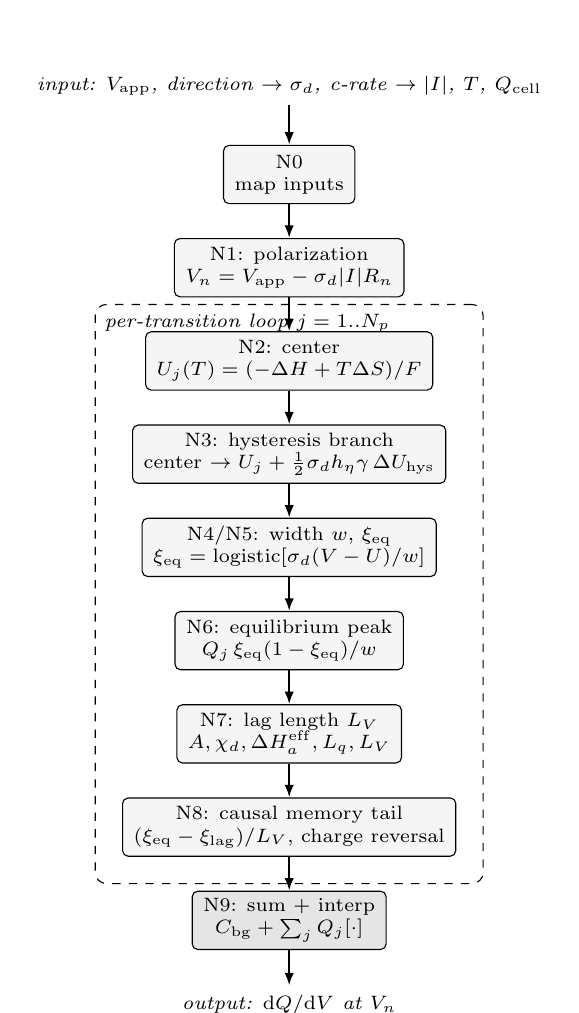
\begin{tikzpicture}[
  node distance=4.3mm and 5.5mm,
  stage/.style={draw,rounded corners=2pt,minimum height=7.4mm,inner xsep=4pt,inner ysep=2.5pt,font=\scriptsize,align=center,fill=black!4},
  core/.style={stage,fill=black!10},
  io/.style={font=\scriptsize\itshape,align=center},
  ar/.style={-{Latex[length=1.6mm]},thick}]
% input row
\node[io] (in) {input: $V_\app$, direction $\to\sigma_d$, c-rate $\to|I|$, $T$, $Q_\cell$};
% spine
\node[stage,below=5mm of in] (n0) {N0\\map inputs};
\node[stage,below=of n0] (n1) {N1: polarization\\$V_n=V_\app-\sigma_d|I|R_n$};
\node[stage,below=of n1] (n2) {N2: center\\$U_j(T)=(-\Delta H+T\Delta S)/F$};
\node[stage,below=of n2] (n3) {N3: hysteresis branch\\center $\to U_j+\tfrac12\sigma_d h_\eta\gamma\,\Delta U_\hys$};
\node[stage,below=of n3] (n4) {N4/N5: width $w$, $\xi_\eq$\\$\xi_\eq=\mathrm{logistic}[\sigma_d(V-U)/w]$};
\node[stage,below=of n4] (n6) {N6: equilibrium peak\\$Q_j\,\xi_\eq(1-\xi_\eq)/w$};
\node[stage,below=of n6] (n7) {N7: lag length $L_V$\\$A,\chi_d,\Delta H_a^\eff,L_q,L_V$};
\node[stage,below=of n7] (n8) {N8: causal memory tail\\$(\xi_\eq-\xi_\mathrm{lag})/L_V$, charge reversal};
\node[core,below=of n8] (n9) {N9: sum + interp\\$C_\bg+\sum_j Q_j[\cdot]$};
\node[io,below=4.5mm of n9] (out) {output: $\dd Q/\dd V$ at $V_n$};
\foreach \a/\b in {in/n0,n0/n1,n1/n2,n2/n3,n3/n4,n4/n6,n6/n7,n7/n8,n8/n9,n9/out}
  \draw[ar] (\a) -- (\b);
% per-transition loop bracket
\begin{scope}[on background layer]
\node[draw,dashed,rounded corners,fit=(n2)(n3)(n4)(n6)(n7)(n8),inner sep=3.4mm,label={[font=\scriptsize\itshape,anchor=north west]north west:per-transition loop $j=1..N_p$}] (loop) {};
\end{scope}
\end{tikzpicture}
\caption{[Origin: v7-11 candidate] 한 곡선을 그리는 코드 진행(spine). 외부 실험조건이 \code{curve} facade 에서 $(\sigma_d,|I|,T,Q_\cell)$
로 환산($\mathrm N0$)되어 코어 \code{dqdv} 로 들어가고, 분극으로 내부 전위 $V_n$ 을 얻은 뒤($\mathrm N1$),
전이 $j$ 마다 평형 중심$\cdot$히스 분기$\cdot$폭$\cdot$평형 점유$\cdot$평형 peak$\cdot$지연 길이$\cdot$인과 꼬리를
계산해($\mathrm N2$--$\mathrm N8$) 합산$\cdot$역보간한다($\mathrm N9$). 본 문건의 절 번호가 이 노드 순서다.
점선 상자가 코드의 전이 루프(\code{for tr in transitions}).}
\label{fig:spine}
\end{figure}



\begin{figure}[t]
\centering
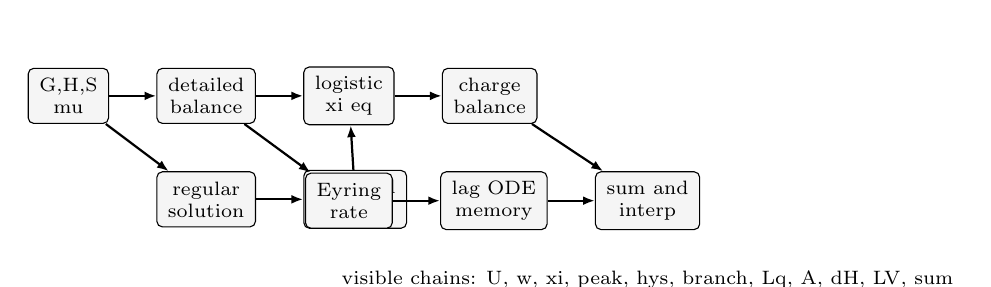
\begin{tikzpicture}[
  node distance=6mm and 6mm,
  box/.style={draw,rounded corners=2pt,fill=black!4,minimum height=7mm,inner xsep=4pt,font=\scriptsize,align=center},
  ar/.style={-{Latex[length=1.5mm]},thick}]
\node[box] (g) {G,H,S\\mu};
\node[box,right=of g] (db) {detailed\\balance};
\node[box,right=of db] (log) {logistic\\xi eq};
\node[box,right=of log] (peak) {charge\\balance};
\node[box,below=of db] (spin) {regular\\solution};
\node[box,right=of spin] (hys) {spinodal\\gap};
\node[box,below=of log] (rate) {Eyring\\rate};
\node[box,right=of rate] (lag) {lag ODE\\memory};
\node[box,right=of lag] (sum) {sum and\\interp};
\draw[ar] (g) -- (db);
\draw[ar] (db) -- (log);
\draw[ar] (log) -- (peak);
\draw[ar] (spin) -- (hys);
\draw[ar] (rate) -- (lag);
\draw[ar] (lag) -- (sum);
\draw[ar] (g) -- (spin);
\draw[ar] (peak) -- (sum);
\draw[ar] (hys) -- (log);
\draw[ar] (db) -- (rate);
\node[font=\scriptsize,align=center,below=4mm of sum] {visible chains: U, w, xi, peak, hys, branch, Lq, A, dH, LV, sum};
\end{tikzpicture}
\caption{[Origin: v8-08 new] v8-08 유도 복원 지도. 그림 내부 텍스트는 영어 ASCII 로 제한했다. 위 행은 열역학과 detailed balance 에서 logistic 과 평형 peak 로 가는 사슬, 가운데는 정규용액 spinodal 에서 히스테리시스 분기로 가는 사슬, 아래는 Eyring 속도에서 지연 ODE, 인과 기억, 최종 합산으로 가는 사슬이다.}
\label{fig:derivechain}
\end{figure}

\tableofcontents
\newpage

% ====================================================================
\section{기호와 규약, 실험조건 매핑 (N0)}\label{sec:notation}
% ====================================================================
계산의 진입점은 facade \code{curve}$(V_\app,\text{direction},\text{c\_rate},Q_\cell,T)$ 이고, 그 첫 일은 실험조건을
코어 \code{dqdv} 의 모델 입력으로 환산하는 것이다 — 이것이 노드 $\mathrm N0$ 다. 방향 문자열은 방향 부호 $\sigma_d$ 로,
C-rate 는 전류 크기 $|I|$ 로 바뀐다:
\begin{equation}
\sigma_d=\begin{cases}+1 & \text{방전(discharge)}\\ -1 & \text{충전(charge)}\end{cases},
\qquad
|I|=\text{c\_rate}\cdot Q_\cell\quad(\text{또는 }I_\mathrm{abs}\text{ 직접 지정}).
\label{eq:n0map}
\end{equation}
방향 부호의 작용처는 셋 — 분극 부호($\mathrm N1$), 분기 중심 선택($\mathrm N3$), 꼬리 지지 방향($\mathrm N8$) — 이며,
평형 종 자체는 방향 불변이다(아래에서 식으로 회수). 본 장이 뽑는 양은 $\dd Q/\dd V$ 한 곡선이다.

\textbf{전이 인덱스.} $j=1,\dots,N_p$($N_p\approx3$--$4$). 전이 $j$ 의 진행률 $\xi_j$(방전 시 $0\to1$ 로 증가, 곧 탈리튬화 진행),
용량 가중 $Q_j$. 박스 결과식은 $j$ 첨자를 단다.

\textbf{부호 규약(★최우선 결함 클래스).} 전위는 흑연 음극 반쪽전지 전위(vs Li/Li$^+$)다. 방향 부호 $\sigma_d=\pm1$
(방전 $+1$/충전 $-1$)이 코드의 \code{s} 인자이며, 평형 점유 $\xi_\eq=\mathrm{logistic}[\sigma_d(V-U)/w]$ 에서 방전
($\sigma_d=+1$)은 $V\!\uparrow\Rightarrow\xi_\eq\!\uparrow$(전위를 올리면 탈리튬화). 분기 중심 $\pm\tfrac12\sigma_d(\cdots)$
는 방전$\cdot$충전이 반대로 갈리고, 꼬리는 충전에서 격자 역전을 받는다. 이 규약은 \S\ref{sec:notation}--\S\ref{sec:sum}
전건에서 유지되며 \S\ref{sec:signcheck} 가 전수 검산한다.

\begin{longtable}{p{0.17\textwidth} p{0.16\textwidth} p{0.585\textwidth}}
\toprule 기호(코드 식별자) & 단위 & 의미 \\ \midrule \endhead
\multicolumn{3}{l}{\emph{— 실험조건$\cdot$방향(N0$\cdot$N1) —}}\\
$\sigma_d$ (\code{s},\,\code{sigma\_d}) & --- & 방향 부호 — 방전 $+1$/충전 $-1$ \\
$|I|$ (\code{I\_abs}) & A & 전류 크기 $=$ c\_rate$\cdot Q_\cell$ \\
$Q_\cell$ (\code{Q\_cell}) & C & 셀 용량(전하); $q=Q/Q_\cell$ 환산$\cdot$$|I|$ 환산 공용 \\
$T$ (\code{T}) & K & 온도 — 스칼라(등온) 또는 $V_\app$ 길이 배열($T(V)$ 비등온) \\
$R_n$ (\code{Rn}) & $\Omega$ & 음극 lumped 분극 저항 \\
$V_\app$ (\code{V\_app}) & V & 인가(측정) 전위 격자 \\
$V_n$ & V & 내부(열역학) 전위 $=V_\app-\sigma_d|I|R_n$ \\
\multicolumn{3}{l}{\emph{— 평형 중심$\cdot$폭$\cdot$점유(N2$\cdot$N4$\cdot$N5) —}}\\
$U_j(T)$ (\code{U},\,\code{func\_U\_j}) & V & 전이 $j$ 평형 중심 전위 $=(-\Delta H_\rxn+T\Delta S_\rxn)/F$ \\
$\Delta H_{\rxn,j},\Delta S_{\rxn,j}$ (\code{dH\_rxn},\code{dS\_rxn}) & {\footnotesize J/mol;\,J/(mol\,K)} & 삽입 \emph{반응} 엔탈피$\cdot$엔트로피(평형 — \emph{활성화}와 다름) \\
$n_j$ (\code{n}) & --- & 폭 다중도($w=n_jRT/F$; \code{w} 주면 $n=wF/RT$ 역산) \\
$w_j$ (\code{func\_w}/\code{func\_w\_eff}) & V & 전이 폭 척도 $=n_jRT/F$(옵션 $w^\eff$) \\
$\xi_{\eq,j}$ (\code{func\_ksi\_eq}) & --- & 평형 진행률(logistic) \\
$Q_j$ (\code{Q}) & C & 전이 $j$ 용량 가중 \\
$C_\bg$ (\code{Cbg}) & C/V & 배경 미분용량(상수 또는 $V$ 함수) \\
\multicolumn{3}{l}{\emph{— 히스테리시스 분기(N3) —}}\\
$\Omega_j$ (\code{Omega}) & J/mol & 정규용액 상호작용 에너지($>2RT$ 면 상분리$\cdot$히스) \\
$\gamma_j$ (\code{gamma}) & --- & 분기 축소 인자 $0\le\gamma_j\le1$($0$ 이면 분기 없음) \\
$\Delta U_j^\hys$ (\code{func\_dU\_hys}) & V & spinodal 상한 분기 gap \\
$h_{\eta,j}$ (\code{h\_eta}) & --- & 부분 cycle 인자(기본 $1$) \\
$U_j^{\,d}$ (\code{center},\,\code{func\_U\_branch}) & V & 방향별 분기 중심 \\
\multicolumn{3}{l}{\emph{— 동역학 꼬리(N7$\cdot$N8) —}}\\
$\chi$ (\code{chi},\,\code{x}) & --- & 전이상태 분율 위치(전달 계수); 방향별 $\chi_d$ \\
$\chi_d$ (\code{func\_chi\_d}) & --- & 방향별 전달 계수 — 방전 $\chi$/충전 $1-\chi$ \\
$\mathcal A$ (\code{A}) & J/mol & 꼬리 컷점 affinity $=\min(z_\mathrm{cut}n_jRT,\,A_\mathrm{cap}RT)$ \\
$\Delta H_{a,j},\Delta S_{a,j}$ (\code{dH\_a},\code{dS\_a}) & {\footnotesize J/mol;\,J/(mol\,K)} & \emph{활성화} 엔탈피$\cdot$엔트로피(속도) \\
$\Delta H_{a,j}^\eff$ (\code{func\_dH\_a\_eff}) & J/mol & 유효 장벽 $=\Delta H_a-\chi_d\Omega$ \\
$L_{q,j}$ (\code{func\_L\_q}) & --- & 용량축 지연 길이 \\
$L_{V,j}$ (\code{lag\_len\_V}) & V & 전압축 지연 길이 $=|\dd V/\dd q|_{q_a}L_{q,j}$ \\
$|\dd V/\dd q|_{q_a}$ (\code{dVdq\_qa}) & V & 컷점 OCV 기울기($L_q\to L_V$ 환산) \\
$z_\mathrm{cut}$ (\code{z\_cut}) & --- & 컷 affinity 의 $z=\mathcal A/(n_jRT)$(기본 $4.357$) \\
$A_\mathrm{cap}$ (\code{A\_cap\_RT}) & --- & 컷 affinity 상한 배수(기본 $4.0$) \\
$\xi_{\mathrm{lag},j}$ (\code{occ\_lagged}) & --- & 인과 저역통과된 진행률 \\
\multicolumn{3}{l}{\emph{— 상수 —}}\\
$R,F,k_B,h$ & {\footnotesize J/(mol\,K), C/mol, J/K, J\,s} & 기체상수, Faraday, Boltzmann, Planck \\
\bottomrule
\end{longtable}

흑연 staging 의 갤러리 채움을 그림~\ref{fig:staging} 에 둔다 — 각 stage 전이가 한 peak 를 남기고, 코드의 전이 리스트
\code{GRAPHITE\_STAGING\_LIT}(4건)이 이 네 전이의 초기값이다.

\begin{figure}[t]
\centering
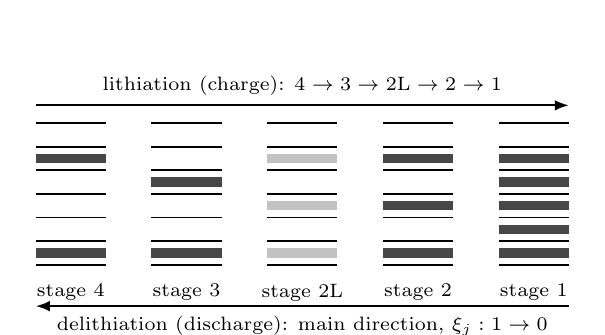
\begin{tikzpicture}[x=1.05cm,y=0.5cm,
  lab/.style={font=\scriptsize,align=center},
  fill4/.style={fill=black!72},fillL/.style={fill=black!24}]
% five stage columns, each shows graphene layers (lines) and Li-filled galleries (bands)
% column x-centers
\def\colw{0.85}
% stage 4: 1 filled gallery of 4
\foreach \x/\name/\filled/\style in {0/{stage 4}/{1}/fill4, 1.4/{stage 3}/{1}/fill4, 2.8/{stage 2L}/{all}/fillL, 4.2/{stage 2}/{all}/fill4, 5.6/{stage 1}/{dense}/fill4}{
  \draw[semithick] (\x,0)--(\x+\colw,0);
  \foreach \k in {1,2,3,4,5,6}{\draw[semithick] (\x,0.6*\k)--(\x+\colw,0.6*\k);}
  \node[lab,below] at (\x+\colw/2,-0.25) {\name};
}
% galleries (bands between layers) — explicit per column for clarity
% stage 4: every 4th gallery filled
\foreach \k in {1,5}{\fill[black!72] (0,0.6*\k-0.42) rectangle (0+\colw,0.6*\k-0.18);}
% stage 3: every 3rd
\foreach \k in {1,4}{\fill[black!72] (1.4,0.6*\k-0.42) rectangle (1.4+\colw,0.6*\k-0.18);}
% stage 2L: every 2nd, light (liquid-like)
\foreach \k in {1,3,5}{\fill[black!24] (2.8,0.6*\k-0.42) rectangle (2.8+\colw,0.6*\k-0.18);}
% stage 2: every 2nd, dark
\foreach \k in {1,3,5}{\fill[black!72] (4.2,0.6*\k-0.42) rectangle (4.2+\colw,0.6*\k-0.18);}
% stage 1: all galleries
\foreach \k in {1,2,3,4,5}{\fill[black!72] (5.6,0.6*\k-0.42) rectangle (5.6+\colw,0.6*\k-0.18);}
\draw[-{Latex[length=1.8mm]},thick] (0,4.05)--(6.45,4.05) node[pos=0.5,above,font=\scriptsize] {lithiation (charge): $4\to3\to2\mathrm L\to2\to1$};
\draw[{Latex[length=1.8mm]}-,thick] (0,-1.05)--(6.45,-1.05) node[pos=0.5,below,font=\scriptsize] {delithiation (discharge): main direction, $\xi_j:1\to0$};
\end{tikzpicture}
\caption{[Origin: v7-11 candidate] 흑연 staging 의 갤러리 채움 도식(신규). 수평선이 그래핀 층, 음영 띠가 리튬이 든 층간 갤러리다.
채울수록 stage 번호가 줄어 stage 1($\mathrm{LiC_6}$, 완전 채움)에 닿고, 각 stage 전이가 $\dd Q/\dd V$ 에 peak
하나를 남긴다. stage $2\mathrm L$ 은 면내 질서가 풀린 단계라 옅게 표시했다. 코드의 전이 리스트 4건이 이 전이들의
초기값이며($U\approx0.21/0.14/0.12/0.085$ V), 본 문건 방향은 방전(탈리튬화)이다.}
\label{fig:staging}
\end{figure}

% ====================================================================
\section{분극 — 측정 전위에서 내부 전위로 (N1)}\label{sec:pol}
% ====================================================================
코어 \code{dqdv} 의 첫 식은 분극을 벗기는 환산이다. 관측은 유한 전류에서 이루어지므로 측정 전위 $V_\app$ 에는 셀의
직렬 저항을 통과한 IR 분극이 실려 있고, 평형 열역학이 사는 전위는 그 분극을 벗긴 내부 전위 $V_n$ 이다.

\subsection{분극 부호 — 방향이 결정한다}
전류 크기 $|I|$ 가 lumped 저항 $R_n$ 을 통과하며 만드는 전위 강하가 $|I|R_n$ 이고, 그 부호는 전류 방향이 정한다.
방전($\sigma_d=+1$)은 음극에서 산화(탈리튬화)가 일어나는 방향이라 측정 전위가 내부 전위보다 분극만큼 \emph{높게}
관측되므로, 내부 전위는 그만큼 낮춰 읽어야 한다. 충전($\sigma_d=-1$)은 부호가 반대다. 두 경우를 한 식으로 묶으면

\begin{derivebox}
\textbf{분극식 유도.} 내부 전위와 측정 전위의 차이는 lumped 저항에서 생기는 IR 항 하나로 둔다. 전류 방향을 부호로 분리하면
\begin{equation*}
  V_{\app}-V_n=\sigma_d |I|R_n .
\end{equation*}
방전은 산화 방향이라 $\sigma_d=+1$ 이고 측정 전위가 내부 전위보다 높다. 충전은 같은 크기의 항이 반대 부호로 붙는다. 양변을 $V_n$ 에 대해 풀면 한 줄 보정식이 된다.
\end{derivebox}

\begin{equation}
\boxed{\;V_n\;=\;V_\app\;-\;\sigma_d\,|I|\,R_n\;.}
\label{eq:vn}
\end{equation}
이것이 코드의 \code{V\_n = V\_in - sigma\_d * I\_abs * self.Rn} 한 줄이다. 부호 약속을 식으로 확인하면 —
방전에서 $V_n=V_\app-|I|R_n<V_\app$(측정이 내부보다 높음), 충전에서 $V_n=V_\app+|I|R_n>V_\app$ — 이며,
$|I|\to0$ 또는 $R_n=0$ 에서 $V_n=V_\app$ 로 두 전위가 일치한다.

\subsection{작업 격자 — 꼬리가 들어올 여유}
이후 모든 전이 계산은 $V_n$ 을 직접 쓰지 않고, $V_n$ 의 범위를 양쪽으로 넓힌 균일 \emph{작업 격자} $V_\work$ 위에서
이루어진다. 넓힘은 동역학 꼬리(\S\ref{sec:tail})가 격자 밖에서 잘려 인공 절단이 생기지 않도록 하는 여유다.
$v_\mathrm{lo}=\min V_n$, $v_\mathrm{hi}=\max V_n$, $\Delta v=v_\mathrm{hi}-v_\mathrm{lo}$ 로
\begin{equation}
V_\work=\mathrm{linspace}\big(v_\mathrm{lo}-p_\mathrm{lo}\,\Delta v,\;
v_\mathrm{hi}+p_\mathrm{hi}\,\Delta v,\;n_\work\big),
\qquad \Delta_\mathrm{grid}=V_{\work,1}-V_{\work,0},
\label{eq:vwork}
\end{equation}
패딩 $p_\mathrm{lo}=p_\mathrm{hi}=0.15$, 점 수 $n_\work=\max(2048,\,2\,|V_n|)$ 이다(코드 \code{grid\_pad\_lo/hi},
\code{n\_work\_min}). 온도가 배열 $T(V)$ 이면 같은 격자 위로 보간해 $T_\work$ 를 얻고($T_\mathrm{rep}=\overline{T_\work}$ 는
전이당 상수 평가용 대표 온도), 스칼라면 $T_\work\equiv T$ 다. 배경은 작업 격자 위에서 먼저 깔린다:
$\dd Q/\dd V|_\work \leftarrow C_\bg(V_\work)$. 모든 전이 기여는 여기에 더해지고($\mathrm N9$), 마지막에 $V_n$ 으로
역보간된다.

\begin{keybox}
\textbf{세 전위.} $V_\app$(측정)$\cdot$$V_n$(내부, 식~\eqref{eq:vn})$\cdot$$V_\work$(계산 격자, 식~\eqref{eq:vwork})는
지위가 다르다. 다음 절부터 평형$\cdot$동역학은 $V_\work$ 위에서 풀고, 출력만 $V_n$ 으로 되돌린다.
\end{keybox}

다음 절은 전이 루프의 첫 식 — 평형 중심 $U_j(T)$ — 으로 들어간다.

% ====================================================================
\section{평형 중심 $U_j(T)$ — 열역학에서 (N2)}\label{sec:center}
% ====================================================================
전이 루프 안의 첫 물리량은 전이 $j$ 의 평형 중심 전위 $U_j(T)$ 다. 코드는 이를 열역학 입력 $(\Delta H_\rxn,\Delta S_\rxn)$
에서 \code{func\_U\_j} 로 계산하거나(없으면) \code{'U'} 를 직접 읽는다. 이 절은 그 환산식이 어디서 오는지를 닫는다.

\subsection{$G,\mu$ 와 평형 조건}
등온$\cdot$등압 계(전지)의 자발성$\cdot$평형을 판정하는 퍼텐셜은 Gibbs 자유에너지 $G\equiv H-TS$ 이고, 입자 1몰 변화당
$G$ 변화가 화학퍼텐셜 $\mu\equiv\partial G/\partial n|_{T,P}$ 다. 두 장소의 $\mu$ 일치가 입자 교환 평형이다. 삽입 반응
$\mathrm{Li}^++e^-+[\,]\rightleftharpoons\mathrm{Li}_{(\text{흑연})}$ 의 전기화학 평형에서, 전자 항이 측정 전위 $V$ 를
통해 $-FV$ 로 들어오므로 평형 조건은
\begin{equation}
\mu_\mathrm{Li}(\theta_\eq)\;=\;\mu^0-sF\,(V-U),
\qquad \Delta G_j\;=\;-sF\,U_j
\label{eq:eqcond}
\end{equation}
형태가 된다($s$ 는 방전 규약 $+1$; $U$ 는 비배치 몫 자유에너지의 전위 환산). 부호의 핵심은 $\Delta G_j=-sFU_j$ —
$U_j$ 가 양이면 $\Delta G_j<0$, 곧 전이가 자발 진행할 전위가 양의 중심이다.

\subsection{$U_j(T)$ — 온도 환산}
$\Delta G_j=\Delta H_{\rxn,j}-T\Delta S_{\rxn,j}$ 를 식~\eqref{eq:eqcond} 의 $\Delta G_j=-sFU_j$($s=+1$)에 적용해 $U_j$ 로 풀면

\begin{derivebox}
\textbf{$U_j(T)$ 유도 사슬.} 출발점은 Gibbs 자유에너지와 화학퍼텐셜이다.
\begin{align*}
G&=H-TS, & \mu&\equiv\left(\frac{\partial G}{\partial n}\right)_{T,P}, & \Delta G_j&=\Delta H_{\rxn,j}-T\Delta S_{\rxn,j}.
\end{align*}
삽입 반응의 전기화학 평형에서 전자 전기일은 전위 항으로 묶이며, v11 부호 규약에서는
\begin{equation*}
\mu_{\mathrm{Li}}(\theta_{\eq})=\mu^0-sF(V-U_j),\qquad \Delta G_j=-sF U_j.
\end{equation*}
Chapter 1 의 중심 전위는 방전 기준 $s=+1$ 로 저장된다. 따라서
\begin{equation*}
-FU_j=\Delta H_{\rxn,j}-T\Delta S_{\rxn,j},
\end{equation*}
이고, 양변을 $-F$ 로 나누면 코드의 \code{func\_U\_j} 식이 나온다. 이 사슬은 ``OCV 표에서 읽기''가 아니라 $G\to\mu\to\Delta G=-FU$ 로 내부 전위 중심을 정하는 열역학 환산이다.
\end{derivebox}

\begin{equation}
\boxed{\;U_j(T)\;=\;\frac{-\Delta H_{\rxn,j}+T\,\Delta S_{\rxn,j}}{F}\;.}
\label{eq:Uj}
\end{equation}
이것이 \code{func\_U\_j(T, dH\_rxn, dS\_rxn)} 의 \code{(-dH\_rxn + T*dS\_rxn)/F} 다. 부호 — 발열 반응
$\Delta H_\rxn<0$ 이면 분자 $-\Delta H_\rxn>0$ 이 중심을 \emph{올린다}(흡열 아님에 주의). 온도 의존은
$\partial U_j/\partial T=\Delta S_{\rxn,j}/F$ 이고, $|\Delta S_\rxn|\sim$ 수$\sim$수십 J/(mol\,K) 라 $30$ K 창에서 수 mV
규모로 중심이 이동한다 — 다온도 피팅에서 온도마다 $U_j(T)$ 를 따로 읽어야 하는 이유다. 코드가 배열 $T_\work$ 를 그대로
넣으므로 $U_j$ 는 비등온이면 격자별 배열로 나온다.

\begin{codebox}
\textbf{N2.} \code{if 'dH\_rxn' in tr and 'dS\_rxn' in tr: U\_j = func\_U\_j(T\_work, dH\_rxn, dS\_rxn)}
— 배열 $T_\work$ 대응. 없으면 \code{U\_j = float(tr['U'])} 직접. \code{GRAPHITE\_STAGING\_LIT} 의 stage 2$\to$1 은
$\Delta H_\rxn=-13000$ J/mol, $\Delta S_\rxn=-16$ J/(mol\,K) $\Rightarrow$ $U(298)=(13000-298.15\times16)/96485
\approx0.0853$ V(목표 $0.085$ V 정합).
\end{codebox}

다음은 같은 루프 안에서 이 중심을 충$\cdot$방전으로 갈라놓는 히스테리시스 분기다.

% ====================================================================
\section{히스테리시스 분기 중심 (N3)}\label{sec:hys}
% ====================================================================
코드는 평형 중심 $U_j$ 를 곧바로 쓰지 않고, 상호작용 $\Omega_j$ 와 분기 인자 $\gamma_j$ 가 있으면 방향별 분기 중심
$U_j^{\,d}$ 로 옮긴다. 본 문건의 주 전개는 방전이며, 히스테리시스는 그 위의 \emph{구조적 분기}로 선언된다 — 방전과 충전이
같은 전이를 서로 다른 준안정 가지로 과주행해 중심이 갈라진다. 이 절은 그 gap 의 닫힌 식과 부호를 유도한다.

\subsection{상호작용이 평형을 비트는 곳}
격자기체의 화학퍼텐셜에는 섞임 엔트로피 로그 몫 외에 정규용액 상호작용 몫 $\Omega_j(1-2\theta)$ 가 더해진다($\Omega>0$
이면 동종 이웃 인력). 자유에너지를 진행률 $\xi=1-\theta$ 로 적으면
\begin{equation}
g_j(\xi)=g_j^0+RT\big[\xi\ln\xi+(1-\xi)\ln(1-\xi)\big]+\Omega_j\,\xi(1-\xi),
\label{eq:gxi}
\end{equation}
이고 두 번 미분하면 $g_j''(\xi)=RT/[\xi(1-\xi)]-2\Omega_j$ 다. $g_j''=0$ 의 두 근이 \textbf{spinodal}:
\begin{equation}
\xi_{s,j}^\pm=\tfrac12(1\pm u_j),\qquad
u_j\equiv\sqrt{1-\frac{2RT}{\Omega_j}}\quad(\Omega_j>2RT).
\label{eq:spinodal}
\end{equation}
$u_j$ 가 실수가 되는 조건 $\Omega_j>2RT$ 가 상분리(따라서 히스테리시스)의 문턱이며, $\Omega_j\le2RT$ 면 갈라짐이 없다.
이 문턱이 코드의 명시 분기 \code{if Omega <= 2RT: return 0.0} 이다.

\subsection{gap 의 닫힌 꼴 — 두 spinodal 의 전위 차}
자유에너지~\eqref{eq:gxi} 에서 나온 평형 전위 곡선
$V_{\eq,j}(\xi)=U_j+\frac{RT}{sF}\ln\frac{\xi}{1-\xi}+\frac{\Omega_j}{sF}(1-2\xi)$ 는 $\Omega_j>2RT$ 면
비단조다. 방전은 $\xi\!\approx\!0$ 에서 상승 가지를 극대 $\xi_{s,j}^-$ 까지, 충전은 $\xi\!\approx\!1$ 에서 극소 $\xi_{s,j}^+$
까지 과주행하므로(그림~\ref{fig:hysloop}), 두 극값의 전위 차가 분기 gap 의 spinodal 상한이다.
위 유도 복원 박스의 spinodal 중간식을 두 극값 차에 적용한다. 두 끝점에서
$\xi/(1-\xi)$ 는 서로 역수이고, $(1-2\xi_{s,j}^-)=+u_j$, $(1-2\xi_{s,j}^+)=-u_j$ 이다. 극대에서 극소를 빼면 $U_j$ 가 상쇄되고 로그 차가 $\mathrm{artanh}$ 로 묶여

\begin{derivebox}
\textbf{$\Delta U_j^{\hys}$ 유도 사슬.} 정규용액 자유에너지에서 시작한다.
\begin{equation*}
g_j(\xi)=g_j^0+RT[\xi\ln\xi+(1-\xi)\ln(1-\xi)]+\Omega_j\xi(1-\xi).
\end{equation*}
두 번 미분하면
\begin{equation*}
g_j''(\xi)=\frac{RT}{\xi(1-\xi)}-2\Omega_j.
\end{equation*}
spinodal 은 $g_j''=0$ 이므로 $\xi(1-\xi)=RT/(2\Omega_j)$, 곧 근의 공식으로
\begin{equation*}
\xi_{s,j}^{\pm}=\frac12(1\pm u_j),\qquad u_j=\sqrt{1-\frac{2RT}{\Omega_j}}.
\end{equation*}
평형 전위 곡선은
\begin{equation*}
V_{\eq,j}(\xi)=U_j+\frac{RT}{sF}\ln\frac{\xi}{1-\xi}+\frac{\Omega_j}{sF}(1-2\xi).
\end{equation*}
두 spinodal 에서
\begin{equation*}
\frac{\xi_s^-}{1-\xi_s^-}=\frac{1-u_j}{1+u_j},\quad
\frac{\xi_s^+}{1-\xi_s^+}=\frac{1+u_j}{1-u_j},\quad
1-2\xi_s^-=u_j,\qquad 1-2\xi_s^+=-u_j.
\end{equation*}
극대에서 극소를 빼면 $U_j$ 가 사라지고 로그 차는 $-4\operatorname{artanh}u_j$ 로 정리된다. 방전 기준 $s=+1$ 로 코드가 쓰는 gap 은 아래 박스가 된다.
\end{derivebox}

\begin{equation}
\boxed{\;\Delta U_j^\hys
=\frac{2}{F}\Big[\Omega_j\,u_j-2RT\,\mathrm{artanh}\,u_j\Big],
\qquad u_j=\sqrt{1-\frac{2RT}{\Omega_j}}\;.}
\label{eq:dUhys}
\end{equation}
($s=+1$; $\mathrm{artanh}\,u=\tfrac12\ln\tfrac{1+u}{1-u}$ 로 로그 항을 정리.) 이것이 \code{func\_dU\_hys(T, Omega)} 의
\code{(2/F)*(Omega*u - 2*R*T*arctanh(u))} 이며, $\Omega\le2RT$ 면 $0$ 을 반환한다(제곱근 NaN 영역의 명시 분기).
부호 — 극대 $>$ 극소라 $\Delta U_j^\hys\ge0$ 이고, $\Omega_j\to2RT^+$ 에서 $u_j\to0$, $\Delta U_j^\hys\to0$ 으로
연속이다.

\subsection{방향별 분기 중심 $U_j^{\,d}$}
두 spinodal 끝점의 \emph{평균}은 로그 몫 합과 $(1-2\xi)$ 몫 합이 둘 다 $0$ 이라 정확히 $U_j$ 다 — 분기는 $U_j$
대칭이다. 이 대칭 위에서 실측 분기 중심을 방향별 한 자유도로 적으면

\begin{derivebox}
\textbf{분기 중심 유도 사슬.} 위 spinodal 두 전위의 평균을 잡으면 중심 대칭이 바로 보인다.
\begin{align*}
\frac12[V_{\eq}(\xi_s^-)+V_{\eq}(\xi_s^+)]
&=U_j+\frac{RT}{2sF}\left[\ln\frac{1-u}{1+u}+\ln\frac{1+u}{1-u}\right]
+\frac{\Omega}{2sF}[u+(-u)]\\
&=U_j.
\end{align*}
따라서 spinodal 상한 분기는 $U_j$ 를 중심으로 $\pm\tfrac12\Delta U_j^{\hys}$ 이다. 실제 전극은 핵생성, mosaic 진행, 부분 cycle 때문에 상한 전체를 쓰지 않으므로 축소 인자 $\gamma_j$ 와 부분 cycle 인자 $h_{\eta,j}$ 를 곱한다. 방향은 v11 의 $\sigma_d$ 가 받는다.
\end{derivebox}

\begin{equation}
\boxed{\;U_j^{\,d}\;=\;U_j\;+\;\tfrac12\,\sigma_d\,h_{\eta,j}\,\gamma_j\,\Delta U_j^\hys\;.}
\label{eq:Ubranch}
\end{equation}
이것이 \code{func\_U\_branch(T, U\_j, Omega, gamma, sigma\_d, h\_eta)} 의
\code{U\_j + 0.5*sigma\_d*h\_eta*gamma*func\_dU\_hys(T, Omega)} 다. 부호 — 방전($\sigma_d=+1$)은 중심을 $+$ 쪽,
충전($\sigma_d=-1$)은 $-$ 쪽으로 옮겨 $U_j^{\dis}>U_j^{\chg}$(방전 전위가 충전보다 높다는 관측 일치). $\gamma_j=1$ 이
spinodal 상한, $\gamma_j\to0$ 이 히스 소멸, $h_{\eta,j}$ 가 부분 cycle 보정(기본 $1$)이다.

코드는 전이당 상수인 분기 shift 만 필요하므로, 식~\eqref{eq:Ubranch} 의 $U_j$ 자리에 $0$ 을 넣어 shift 분
$\mathrm{hys\_shift}=\code{func\_U\_branch}(T_\rep,0,\Omega,\gamma,\sigma_d,h_\eta)$ 을 얻고, 배열 중심 $U_j$ 에 더한다:
\begin{equation}
\mathrm{center}=
\begin{cases}
U_j+\tfrac12\sigma_d h_{\eta,j}\gamma_j\Delta U_j^\hys(T_\rep) & \gamma_j\ne0 \text{ 이고 } \Omega_j>0\\[2pt]
U_j & \text{그 외(분기 없음)}.
\end{cases}
\label{eq:center}
\end{equation}
이 \code{center} 가 다음 절 평형 점유 $\xi_\eq$ 의 중심으로 들어간다. 평형 종의 \emph{모양} 자체는 방향 불변이고,
방향이 바꾸는 것은 이 중심의 위치(와 \S\ref{sec:tail} 의 꼬리 방향)뿐이다.

\begin{figure}[t]
\centering
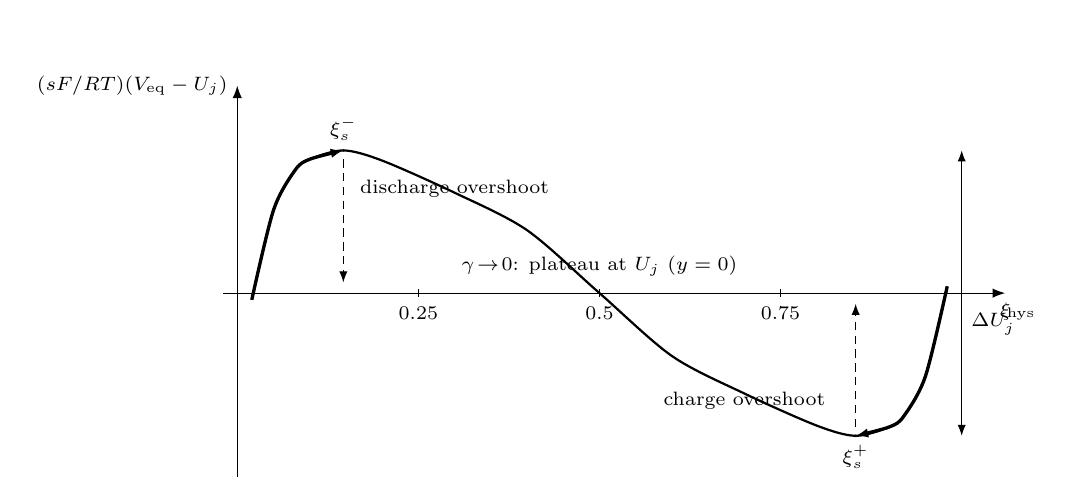
\begin{tikzpicture}[x=9.2cm,y=1.7cm]
\draw[-{Latex[length=1.6mm]}] (0,-1.45) -- (0,1.55) node[left,font=\scriptsize] {$(sF/RT)(V_\eq-U_j)$};
\draw[-{Latex[length=1.6mm]}] (-0.02,0) -- (1.06,0) node[below,font=\scriptsize] {$\xi$};
\foreach \xx in {0.25,0.5,0.75} {\draw (\xx,0.03) -- (\xx,-0.03) node[below,font=\scriptsize] {\xx};}
% non-monotone V_eq(xi) for Omega=4RT (qualitative)
\draw[thick] plot[smooth] coordinates {(0.02,-0.05) (0.05,0.62) (0.08,0.92) (0.1,1.00) (0.1464,1.066) (0.2,0.99) (0.3,0.75) (0.4,0.47) (0.5,0) (0.6,-0.47) (0.7,-0.75) (0.8,-0.99) (0.8536,-1.066) (0.9,-1.00) (0.92,-0.92) (0.95,-0.62) (0.98,0.05)};
\fill (0.1464,1.066) circle (0.5pt) node[above,font=\scriptsize] {$\xi_s^-$};
\fill (0.8536,-1.066) circle (0.5pt) node[below,font=\scriptsize] {$\xi_s^+$};
\draw[{Latex[length=1.4mm]}-{Latex[length=1.4mm]}] (1.0,-1.066) -- (1.0,1.066) node[pos=0.4,right,font=\scriptsize] {$\Delta U_j^\hys$};
% discharge overshoot path (rising branch up to xi_s^-)
\draw[-{Latex[length=1.6mm]},very thick] plot[smooth] coordinates {(0.02,-0.05) (0.05,0.62) (0.08,0.92) (0.1,1.00) (0.1464,1.066)};
\draw[-{Latex[length=1.4mm]},densely dashed] (0.1464,1.0) -- (0.1464,0.08);
\node[font=\scriptsize] at (0.30,0.78) {discharge overshoot};
% charge overshoot path
\draw[-{Latex[length=1.6mm]},very thick] plot[smooth] coordinates {(0.98,0.05) (0.95,-0.62) (0.92,-0.92) (0.9,-1.00) (0.8536,-1.066)};
\draw[-{Latex[length=1.4mm]},densely dashed] (0.8536,-1.0) -- (0.8536,-0.08);
\node[font=\scriptsize] at (0.70,-0.80) {charge overshoot};
\node[font=\scriptsize] at (0.5,0.20) {$\gamma\!\to\!0$: plateau at $U_j$ ($y=0$)};
\end{tikzpicture}
\caption{[Origin: v7-11 candidate] 비단조 평형 전위 $V_\eq(\xi)$($\Omega_j=4RT$)와 과주행. 방전(굵은 경로, 좌상)은 극대 $\xi_s^-$ 까지,
충전(우하)은 극소 $\xi_s^+$ 까지 과주행해 중심이 갈라진다. 두 극값 차가 spinodal 상한 gap $\Delta U_j^\hys$
(식~\eqref{eq:dUhys}), 실측 분기는 $\gamma_j$ 만큼 안쪽(식~\eqref{eq:Ubranch}). $\gamma\to0$ 가역 한계에서
두 경로가 $y=0$ plateau 로 합쳐진다.}
\label{fig:hysloop}
\end{figure}

% ====================================================================
\section{폭과 평형 점유 $\xi_\eq$ (N4, N5)}\label{sec:width}
% ====================================================================
중심이 정해지면 코드는 폭 $w_j$ 와 평형 점유 $\xi_{\eq,j}$ 를 평가한다. 이 둘이 평형 종(다음 절의 peak)의 모양을
결정한다. 평형 등온선은 \S\ref{sec:center} 의 평형 조건을 정$\cdot$역 속도의 균형으로 회수하면 logistic 으로 닫힌다.

\subsection{폭 $w_j$ — 이상 극한과 옵션}
평형 점유의 폭 척도는 이상 극한에서 $w_j=n_jRT/F$ 다($n_j$ 는 폭 다중도):

\begin{derivebox}
\textbf{$w_j$ 유도 사슬.} 이상 격자기체에서는 섞임 자유에너지의 로그 몫이 중심 근방의 전위 기울기를 정한다.
\begin{align*}
\mu_{\mathrm{mix}}(\theta)&=RT\ln\frac{\theta}{1-\theta},
& \xi&=1-\theta,
& \frac{\xi}{1-\xi}&=\exp\!\left[\frac{sF(V-U)}{RT}\right].
\end{align*}
단일 자리 전이는 logit 의 자연 폭이 $RT/F$ 이므로
\begin{equation*}
\xi_{\eq}=\frac{1}{1+\exp[-s(V-U)/(RT/F)]}.
\end{equation*}
여러 등가 자리 또는 staging 전이가 한 관측 전이로 뭉치면 전기 일 $F(V-U)$ 가 $n_j$ 배 완만하게 보이는 현상학적 다중도 $n_j$ 를 둔다. 따라서 logit 분모가
\begin{equation*}
w_j=n_j\frac{RT}{F}
\end{equation*}
로 확장된다. v11 에서 \code{w} 를 직접 주면 같은 식을 $n_j=w_jF/(RT)$ 로 거꾸로 풀어 \code{func\_w(T,n)} 에 넣는다.
\end{derivebox}

\begin{equation}
w_j=\frac{n_jRT}{F}\qquad(\text{기본 폭}),
\label{eq:wbase}
\end{equation}
코드 \code{func\_w(T, n)} 의 \code{n*R*T/F}
가 이것이고, 전이 dict 가 \code{'w'} 를 직접 주면 $n_j=w_jF/(RT)$ 로 역산해(\code{\_n\_factor}) 같은 식에 넣는다.
상호작용이 종을 좁히는 옵션 유효 폭은
\begin{equation}
w_j^\eff=\frac{RT}{F}\Big(1-\frac{\Omega_j}{2RT}\Big),
\label{eq:weff}
\end{equation}
이며 $\Omega_j\to2RT$ 에서 $0$ 으로 가므로 코드는 $\mathrm{floor\_frac}\cdot RT/F$ 하한으로 클립한다(\code{func\_w\_eff},
기본 \code{w\_eff\_floor\_frac}$=0.05$). 이 좁힘은 명시적으로 \code{use\_w\_eff} 를 켤 때만 적용되고, 기본은
$w_j=n_jRT/F$ 다(\code{\_width}).

\subsection{평형 점유 $\xi_\eq$ — logistic 의 유도}
정$\cdot$역 두 방향 속도가 같은 정지점에서 점유비가 Boltzmann 비 $e^{\mathcal A_j/RT}$ 와 같다는 detailed balance 로부터,
구동력 $\mathcal A_j=sF(V_n-U_j)$ 를 넣고 진행률에 대해 풀면 평형 등온선이 logistic 으로 닫힌다:

\begin{derivebox}
\textbf{$\xi_{\eq}$ logistic 유도 사슬.} 정방향과 역방향 속도는 같은 전이상태를 지나며 affinity $\mathcal A_j$ 가 장벽을 비대칭으로 이동시킨다.
\begin{align*}
r_j^+&=k_0\exp\!\left[-\frac{\Delta G_{a,j}-\chi\mathcal A_j}{RT}\right],\qquad
r_j^-=k_0\exp\!\left[-\frac{\Delta G_{a,j}+(1-\chi)\mathcal A_j}{RT}\right],\\
\frac{r_j^+}{r_j^-}&=\exp\!\left[\frac{\mathcal A_j}{RT}\right].
\end{align*}
정지점에서는 찬 자리에서 출발하는 정방향 사건과 빈 자리에서 출발하는 역방향 사건이 같아야 하므로
\begin{equation*}
r_j^+(1-\xi)=r_j^-\xi
\quad\Longrightarrow\quad
\frac{\xi}{1-\xi}=\frac{r_j^+}{r_j^-}=\exp\!\left[\frac{\mathcal A_j}{RT}\right].
\end{equation*}
기본 구동력은 $\mathcal A_j=\sigma_d F(V-U_j^{\,d})$ 이고, 폭 다중도는 $RT/F\mapsto w_j=n_jRT/F$ 로 들어간다. 따라서
\begin{equation*}
\xi=\frac{\exp[\sigma_d(V-U_j^{\,d})/w_j]}{1+\exp[\sigma_d(V-U_j^{\,d})/w_j]}
=\frac{1}{1+\exp[-\sigma_d(V-U_j^{\,d})/w_j]}.
\end{equation*}
\end{derivebox}

\begin{equation}
\boxed{\;\xi_{\eq,j}(V,T)=\frac{1}{1+\exp\!\big[-\sigma_d(V-U_j^{\,d})/w_j\big]}\;.}
\label{eq:xieq}
\end{equation}
폭 다중도 $n_j$ 는 식~\eqref{eq:wbase} 의 $w_j=n_jRT/F$ 로 logistic 인자의 분모에 들어간다(detailed balance 가 닫는 $RT/F$ 의 폭 다중도 일반화). 방향 부호가 logistic 인자의 부호로 들어간다 — 이것이 \code{func\_ksi\_eq(T, V\_n, U, n, s)} 의
$z=\sigma_d(V_\work-U_j^{\,d})/w_j$(폭은 \code{func\_w}$(T,n)$)이며, 코드는 오버플로 방지를 위해 $z\ge0$ 과 $z<0$ 을
갈라 평가한다(\code{np.where(z>=0, 1/(1+e\^{-z}), e\^{z}/(1+e\^{z}))} — 수학적으로 동일). 여기서 평가 전위는
내부 전위 $V_n$ 이 아니라 \S\ref{sec:pol} 의 작업 격자 $V_\work$ 다 — 코드 호출 \code{func\_ksi\_eq(T\_work,
V\_work, center, n\_j, sigma\_d)} 에서 함수의 \code{V\_n} 인자 자리에 $V_\work$ 가 들어간다(평형$\cdot$동역학은
$V_\work$ 위에서 풀고 출력만 $V_n$ 으로 역보간하는 규약, 식~\eqref{eq:vwork}). 호출 시 중심 $U_j^{\,d}$ 는
식~\eqref{eq:center} 의 \code{center}(분기 있으면 분기 중심, 없으면 $U_j$)다.

\begin{signbox}
\textbf{부호.} 방전 $\sigma_d=+1$: $V\!\uparrow\Rightarrow z\!\uparrow\Rightarrow\xi_\eq\!\uparrow$ — 전위를 올리면
탈리튬화 진행이 는다(규약 일치). 충전 $\sigma_d=-1$: $V\!\uparrow\Rightarrow z\!\downarrow\Rightarrow\xi_\eq\!\downarrow$.
극한 — $V\gg U_j^{\,d}\Rightarrow\xi_\eq\to1$(방전), $V\ll U_j^{\,d}\Rightarrow0$, $V=U_j^{\,d}\Rightarrow\tfrac12$
(전이 중심). $w_j=RT/F=25.7$ mV($25^\circ$C).
\end{signbox}

그림~\ref{fig:logistic} 가 $\xi_\eq$ 와 그 미분(다음 절의 종)을 함께 보인다. 다음 절은 이 종이 평형 peak 임을 닫는다.

\begin{figure}[t]
\centering
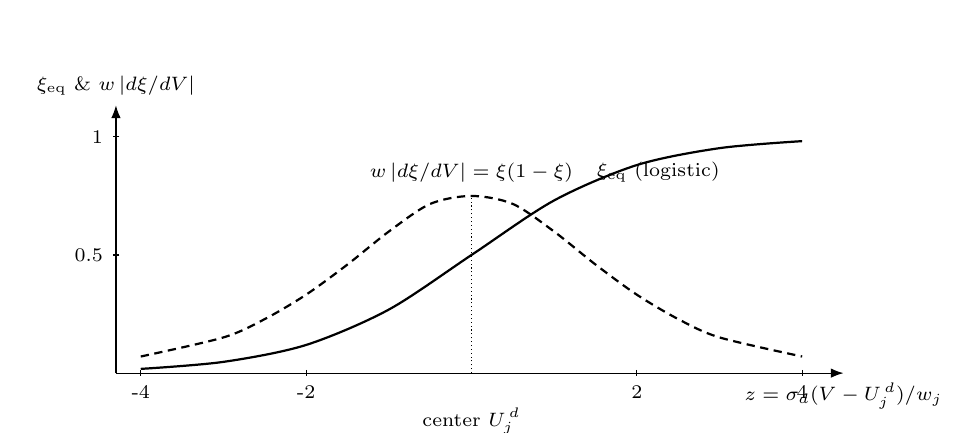
\begin{tikzpicture}[x=1.05cm,y=1.0cm]
% left axis: xi_eq (S-curve), right: dxi/dV bell — shared z-axis
\draw[-{Latex[length=1.6mm]}] (-4.3,0) -- (4.5,0) node[below,font=\scriptsize] {$z=\sigma_d(V-U_j^{\,d})/w_j$};
\draw[-{Latex[length=1.6mm]}] (-4.3,0) -- (-4.3,3.4) node[above,font=\scriptsize] {$\xi_\eq$ \&\ $w\,|d\xi/dV|$};
\foreach \xx in {-4,-2,2,4} {\draw (\xx,0.04) -- (\xx,-0.04) node[below,font=\scriptsize] {\xx};}
\draw (-4.26,3.0) -- (-4.34,3.0) node[left,font=\scriptsize] {1};
\draw (-4.26,1.5) -- (-4.34,1.5) node[left,font=\scriptsize] {0.5};
% xi_eq = 1/(1+e^-z) scaled by 3
\draw[thick] plot[smooth] coordinates {(-4,0.0537) (-3,0.1429) (-2,0.3577) (-1,0.8068) (0,1.5) (1,2.1932) (2,2.6423) (3,2.8571) (4,2.9463)};
\node[right,font=\scriptsize] at (1.4,2.55) {$\xi_\eq$ (logistic)};
% derivative xi(1-xi) max 0.25 scaled by 12 -> max 3
\draw[densely dashed,thick] plot[smooth] coordinates {(-4,0.211) (-3,0.4534) (-2.5,0.6864) (-2,0.9963) (-1.5,1.3792) (-1,1.7976) (-0.5,2.1487) (0,2.25) (0.5,2.1487) (1,1.7976) (1.5,1.3792) (2,0.9963) (2.5,0.6864) (3,0.4534) (4,0.211)};
\node[font=\scriptsize] at (0,2.55) {$w\,|d\xi/dV|=\xi(1-\xi)$};
\draw[densely dotted] (0,0)--(0,2.25);
\node[below,font=\scriptsize] at (0,-0.32) {center $U_j^{\,d}$};
\end{tikzpicture}
\caption{[Origin: v7-11 candidate] 평형 점유와 그 미분(신규). 실선 $=\xi_\eq$ logistic(식~\eqref{eq:xieq}), 파선 $=$ 폭으로 규격화한 미분
$w_j|d\xi_\eq/dV|=\xi_\eq(1-\xi_\eq)$ — $z=0$(중심 $U_j^{\,d}$)에서 최대 $\tfrac14$ 인 종 모양. 이 종이
다음 절의 평형 peak 이고, 방향에 불변(양수)이다.}
\label{fig:logistic}
\end{figure}

% ====================================================================
\section{평형 peak — $|I|\to0$ 기준선 (N6)}\label{sec:eqpeak}
% ====================================================================
코드는 평형 점유에서 곧바로 평형 peak 모양 $\xi_\eq(1-\xi_\eq)/w$ 를 만든다. 이것이 전류가 없을 때($|I|\to0$)의
기준선이며, 동역학 꼬리가 무시될 만큼 작을 때 코드가 직접 쓰는 항이다.

관측 $\dd Q/\dd V$ 는 전하 보존식 $Q_\cell q=Q_\bg(V_n)+\sum_jQ_j\xi_j$ 를 궤적 $q$ 로 미분해
$\dd Q/\dd V_n=C_\bg+\sum_jQ_j\,\dd\xi_j/\dd V_n$ 으로 닫힌다. 평형 추종이면 $\dd\xi_j/\dd V_n$ 에 평형 기울기가 들어가고,
logistic 미분의 종 항등식 $d\xi_\eq/dz=\xi_\eq(1-\xi_\eq)$ 에 연쇄율 $dz/dV=\sigma_d/w_j$ 를 곱하면
\begin{derivebox}
\textbf{평형 peak 유도 사슬.} 출발식은 내부 전위가 들어간 전하 보존식이다.
\begin{equation*}
Q_\cell q=Q_\bg(V_n)+\sum_jQ_j\xi_j .
\end{equation*}
궤적 $q$ 를 따라 미분하면
\begin{equation*}
Q_\cell=C_\bg\frac{\dd V_n}{\dd q}+\sum_jQ_j\frac{\dd\xi_j}{\dd q},
\end{equation*}
이고, 양변을 $\dd V_n/\dd q$ 로 나누면
\begin{equation*}
\frac{\dd Q}{\dd V_n}=C_\bg+\sum_jQ_j\frac{\dd\xi_j}{\dd V_n}.
\end{equation*}
평형 추종에서는 $z=\sigma_d(V-U_j^{\,d})/w_j$ 와
$\xi_\eq=(1+e^{-z})^{-1}$ 를 쓴다. 이때
\begin{align*}
\frac{\dd\xi_\eq}{\dd z}
&=\frac{e^{-z}}{(1+e^{-z})^2}
=\frac{1}{1+e^{-z}}\frac{e^{-z}}{1+e^{-z}}
=\xi_\eq(1-\xi_\eq),\\
\frac{\dd z}{\dd V}&=\frac{\sigma_d}{w_j}.
\end{align*}
따라서 $\dd\xi_\eq/\dd V=\sigma_d\xi_\eq(1-\xi_\eq)/w_j$ 이고, ICA peak 모양은 그 절댓값을 쓴다.
\end{derivebox}
\begin{equation}
\frac{\dd\xi_{\eq,j}}{\dd V}=\frac{\sigma_d\,\xi_{\eq,j}(1-\xi_{\eq,j})}{w_j}
\;\Longrightarrow\;
\boxed{\;\Big(\frac{\dd Q}{\dd V}\Big)^\eq_j
=Q_j\,\frac{\xi_{\eq,j}(1-\xi_{\eq,j})}{w_j}
=Q_j\,\Big|\frac{\dd\xi_{\eq,j}}{\dd V}\Big|\;.}
\label{eq:eqpeak}
\end{equation}
이것이 코드의 \code{peak\_shape = ksi\_eq * (1 - ksi\_eq) / w} 이며, 메서드 \code{equilibrium} 이 전이별로 이 항만
합산한 것($C_\bg+\sum_jQ_j\xi_\eq(1-\xi_\eq)/w$)이다. 부호 — $\sigma_d$ 가 미분에서 한 번 들어오지만 peak 모양은
절댓값 $|\dd\xi/\dd V|=\xi_\eq(1-\xi_\eq)/w$ 로 양수이고 방향 불변이다($\xi(1-\xi)\ge0$). 세 양 — 위치 $=$ 중심
$U_j^{\,d}$, 순높이 $=Q_j/(4w_j)$($\xi=\tfrac12$ 에서 $\xi(1-\xi)=\tfrac14$), 배경 차감 면적 $=Q_j$
($\int_0^1\dd\xi=1$) — 가 이 한 식에서 읽힌다.

코드의 사용 조건은 ``지연 길이가 격자에 비해 작을 때''다 — 다음 절이 그 지연 길이 $L_V$ 를 세우고, $L_V$ 가 격자
몇 칸보다 작으면(또는 동역학 키가 없으면) 코드는 식~\eqref{eq:eqpeak} 의 평형 종을 직접 쓴다. 이것이 $|I|\to0$ 환원이다.

% ====================================================================
\section{동역학 지연 길이 $L_V$ (N7)}\label{sec:lag}
% ====================================================================
유한 전류에서는 평형 목표 $\xi_\eq$ 를 점유가 즉시 따라가지 못하고 뒤처진다 — 그 지연이 peak 의 꼬리다. 코드는 전이당
하나의 지연 길이 $L_{V,j}$ 를 resolver \code{\_resolve\_lag\_length} 로 구한다. 이 절은 그 사슬
$\mathcal A\to\chi_d\to\Delta H_a^\eff\to L_q\to L_V$ 를 닫는다.

\subsection{지연의 보편 방정식과 용량축 길이 $L_q$}
정전류에서 $\dd q/\dd t=|I|/Q_\cell$ 이므로 운동방정식 $\dd\xi_j/\dd t=k_j(\xi_{\eq,j}-\xi_j)$ 를 $\dd q/\dd t$ 로
나누면, 지연 $r_j\equiv\xi_{\eq,j}-\xi_j$ 가 영역 제한 없이 성립하는 보편 1계 방정식을 따른다:

\begin{derivebox}
\textbf{$L_q$ 유도 사슬.} 정전류에서는 $\dd q/\dd t=|I|/Q_{\cell}$ 이다. 완화식
\begin{equation*}
\frac{\dd\xi_j}{\dd t}=k_j(\xi_{\eq,j}-\xi_j)
\end{equation*}
을 용량축으로 옮기면
\begin{equation*}
\frac{\dd\xi_j}{\dd q}=\frac{Q_{\cell}k_j}{|I|}(\xi_{\eq,j}-\xi_j).
\end{equation*}
지연 $r_j=\xi_{\eq,j}-\xi_j$ 를 미분하면
\begin{equation*}
\frac{\dd r_j}{\dd q}=\frac{\dd\xi_{\eq,j}}{\dd q}-\frac{Q_{\cell}k_j}{|I|}r_j.
\end{equation*}
마지막 계수를 $1/L_{q,j}$ 로 정의하면 $L_{q,j}=|I|/(Q_{\cell}k_j)$ 이며, 지연 길이는 요구 속도와 완화 공급 속도의 비가 된다.
\end{derivebox}

\begin{equation}
\frac{\dd r_j}{\dd q}=\frac{\dd\xi_{\eq,j}}{\dd q}-\frac{r_j}{L_{q,j}},
\qquad L_{q,j}=\frac{|I|}{Q_\cell\,k_j}.
\label{eq:Lq}
\end{equation}
$L_{q,j}$ 는 요구($|I|/Q_\cell$)와 공급($k_j$) 의 비 그 자체다 — 근본식의 세 인자가 전부 이 한 양을 통해 꼬리로
들어온다. 완화 속도 $k_j$ 는 평형 근방 선형 완화에서 정$\cdot$역 속도의 합 $k_j=k^++k^-=k^+\big(1+e^{-\mathcal A_j/RT}\big)$ 다(detailed balance $k^-/k^+=e^{-\mathcal A_j/RT}$); forward $k^+\simeq k_0\exp[-(\Delta G_{a,j}^\eff-\chi_d\mathcal A_j)/RT]$
($k_0=k_BT/h$)을 적용하면, 앞의 $L_q=|I|/(Q_\cell k_j)$ 정의가 코드 평가 형태로 이어진다.

\subsection{컷 affinity $\mathcal A$ — 꼬리 시작점의 구동력}
$L_q$ 는 전이당 한 점(꼬리 컷점 $q_a$)에서 \emph{상수로 동결}된다. 컷점은 원천 $\dd\xi_\eq/\dd q$ 가 정점의 일정 분율
(약 $5\%$)로 떨어지는 좌표이고, 그곳의 구동력은 $\mathcal A=z_\mathrm{cut}\cdot n_jRT$ 다($z_\mathrm{cut}=4.357$ 이
그 미분 $\dd\xi_\eq/\dd q$ 의 $5\%$ 컷에 대응 — 점유 $\xi_\eq$ 자체가 아니라 미분 기준). 상한 $A_\mathrm{cap}RT$ 와 함께

\begin{derivebox}
\textbf{컷 affinity 유도 사슬.} logistic 원천의 꼬리 컷은 $\dd\xi_{\eq}/\dd q$ 가 정점의 약 $5\%$ 로 떨어지는 지점으로 잡는다. $z=\mathcal A/(n_jRT)$ 에 대해
\begin{equation*}
\frac{\dd\xi_{\eq}}{\dd z}=\xi_{\eq}(1-\xi_{\eq}),\qquad
\left.\frac{\dd\xi_{\eq}}{\dd z}\right|_{z=0}=\frac14.
\end{equation*}
따라서 컷 $z_{\mathrm{cut}}$ 은
\begin{equation*}
\xi(z_{\mathrm{cut}})[1-\xi(z_{\mathrm{cut}})]\approx0.05\times\frac14,
\end{equation*}
을 만족하는 상수로 두며, v11 기본값은 $z_{\mathrm{cut}}=4.357$ 이다. 이 값은 전이당 컷점에서 평가되는 상수이고, 곡선 위 모든 $V$ 에 대해 다시 미분하는 함수가 아니다. 그러므로
\begin{equation*}
\mathcal A_{\mathrm{cut}}=z_{\mathrm{cut}}n_jRT
\end{equation*}
에 운영 상한 $A_{\mathrm{cap}}RT$ 를 적용한다. $\partial\ln L_q/\partial V<0$ 는 이 컷 규칙의 물리적 동기이고, 코드 안에서 동결된 $\mathcal A$ 의 실현 미분은 $0$ 이다.
\end{derivebox}

\begin{equation}
\mathcal A=\min\!\big(z_\mathrm{cut}\,n_j\,RT,\;A_\mathrm{cap}\,RT\big),
\qquad z_\mathrm{cut}=4.357,\ A_\mathrm{cap}=4.0\ (\text{기본}).
\label{eq:Acut}
\end{equation}
이것이 코드의 \code{A = min(z\_cut * n\_safe * R*T, A\_cap * R*T)} 다. \emph{부호의 핵심} — 컷 affinity 의 \emph{크기}는
충$\cdot$방전 동일($n_j>0$ 라 항상 양수)이고, 방향은 아래 $\chi_d\cdot\Delta H_a^\eff$ 가 받는다. 방향 부호 $\sigma_d$ 를
$\min$ 내부에 방향 부호를 포함하면 충전에서 음수 상한이 되는 버그가 생기므로, 코드는 $\sigma_d$ 를 크기에서 빼고 방향은 전달 계수로만
주입한다.

\subsection{방향별 전달 계수와 유효 장벽}
전이상태가 정$\cdot$역 장벽을 비대칭으로 가르는 분율 $\chi\in[0,1]$ 의 합-1 제약($\chi+\chi'=1$, detailed balance)에서,
방향별 전달 계수는
\begin{equation}
\chi_d=\chi_\mathrm{split}(\chi,\sigma_d)=
\begin{cases}\chi & \sigma_d\ge0\ (\text{방전})\\ 1-\chi & \sigma_d<0\ (\text{충전}).\end{cases}
\label{eq:chid}
\end{equation}
이것이 \code{func\_chi\_d(chi, sigma\_d)} 이며(생성자 \code{chi\_split} 로 다른 규칙 주입 가능), 깊은 꼬리에서 방전은
$\xi\to1$, 충전은 $\xi\to0$ 거울이라 역방향 장벽의 상수 몫이 같은 $+\Omega$ 로 흡수되는 것을 반영한다. 그 흡수가 유효
장벽이다:

\begin{derivebox}
\textbf{$\Delta H_a^{\eff}$ 유도 사슬.} 상호작용을 포함한 구동력은
\begin{equation*}
\mathcal A_j=\sigma_dF(V-U_j)-\Omega_j(1-2\xi_j)
\end{equation*}
로 쓸 수 있다. 정방향 장벽에는 $-\chi_d\mathcal A_j$ 가 들어가므로
\begin{equation*}
\Delta G_{a,j}-\chi_d\mathcal A_j
=\Delta G_{a,j}-\chi_d\sigma_dF(V-U_j)+\chi_d\Omega_j(1-2\xi_j).
\end{equation*}
깊은 꼬리에서 방전은 $\xi\to1$, 충전은 거울상으로 $\xi\to0$ 이며, 방향별 $\chi_d=\chi$ 또는 $1-\chi$ 로 같은 상수 몫 $+\Omega_j$ 가 장벽 보정에 흡수된다. 따라서 코드가 \code{func\_L\_q} 에 넘기는 활성화 엔탈피는 원래 $\Delta H_a$ 에서 방향별 상호작용 보정을 뺀 값이다.
\end{derivebox}

\begin{equation}
\boxed{\;\Delta H_{a,j}^\eff=\Delta H_{a,j}-\chi_d\,\Omega_j\;.}
\label{eq:dHeff}
\end{equation}
이것이 \code{func\_dH\_a\_eff(dH\_a, Omega, chi\_d)} 이고, 코드는 \code{use\_dH\_eff} 가 꺼져 있으면 보강 없이
$\Delta H_a$ 를 그대로 쓴다(헬퍼 \code{\_chi\_and\_dH\_eff} 가 $(\chi_d,\Delta H_a^\eff)$ 를 한 곳에서 낸다).

\subsection{$L_q$ 의 평가와 전압축 환산 $L_V$}
정$\cdot$역 합 $k_j=k^+(1+e^{-\mathcal A_j/RT})$(분모의 $(1+e^{-\mathcal A_j/RT})$ 가 여기서 온다)와 $k_0=k_BT/h$ 를 식~\eqref{eq:Lq} 에 넣고 $\Delta G_a^\eff=\Delta H_a^\eff-T\Delta S_a$ 로 갈라 적으면,
코드가 평가하는 $L_q$ 가 된다:

\begin{derivebox}
\textbf{$L_q$ 로그식 유도 사슬.} detailed balance 에서 완화 속도는
\begin{equation*}
k_j=k^++k^-=k^+(1+e^{-\mathcal A/RT}).
\end{equation*}
Eyring 식과 전위 장벽 이동을 forward 속도에 적용하면
\begin{equation*}
k^+=\frac{k_BT}{h}\exp\!\left[-\frac{\Delta H_{a,j}^{\eff}-T\Delta S_{a,j}-\chi_d\mathcal A}{RT}\right].
\end{equation*}
이 속도를 $L_q=|I|/(Q_{\cell}k_j)$ 정의와 결합하면
\begin{align*}
L_q&=\frac{|I|h}{Q_{\cell}k_BT}\,
\frac{\exp[(\Delta H_{a,j}^{\eff}-T\Delta S_{a,j}-\chi_d\mathcal A)/RT]}{1+e^{-\mathcal A/RT}}\\
&=\frac{T_*}{T}\,\frac{\exp[(\Delta H_{a,j}^{\eff}-T\Delta S_{a,j})/RT]}{1+e^{-\mathcal A/RT}}e^{-\chi_d\mathcal A/RT},
\qquad T_*\equiv\frac{|I|h}{Q_{\cell}k_B}.
\end{align*}
로그로 보면 v11 의 네 항이 그대로 보인다: $\ln(T_*/T)$, $-\ln(1+e^{-\mathcal A/RT})$, $\Delta G_a^{\eff}/RT$, $-\chi_d\mathcal A/RT$.
\end{derivebox}

\begin{equation}
L_{q,j}=\frac{T_*}{T}\,\frac{\exp\!\big[(\Delta H_{a,j}^\eff-T\Delta S_{a,j})/RT\big]}{1+e^{-\mathcal A/RT}}
\,e^{-\chi_d\mathcal A/RT},
\qquad T_*\equiv\frac{|I|\,h}{Q_\cell\,k_B}.
\label{eq:Lqfull}
\end{equation}
\code{func\_L\_q(T, I, Q\_cell, dH\_a, dS\_a, x, A)} 가 이 로그를
\code{ln\_Lq = ln(T\_attempt/T) - ln(1+e\^{-A/RT}) + dG\_a/RT - x*A/RT} 로 적고($T_\mathrm{attempt}=(I/Q_\cell)h/k_B=T_*$,
$x=\chi_d$, $\dd G_a=\Delta H_a^\eff-T\Delta S_a$) 지수화한다. \emph{암묵 전제 명시} — 식~\eqref{eq:Lqfull} 의
$\Delta H_a^\eff$ 는 \code{func\_L\_q} 의 \code{dH\_a} 인자로 들어가는 값 \code{dH\_a\_use} 이고, 이것은
\code{use\_dH\_eff=True} 일 때만 식~\eqref{eq:dHeff} 의 $\Delta H_a-\chi_d\Omega$ 와 같다 — 꺼져 있으면 그대로
$\Delta H_a$ 다(\code{\_chi\_and\_dH\_eff} 의 분기). 전압축으로 옮기면, 컷점 OCV 기울기를 곱한다:

\begin{derivebox}
\textbf{$L_V$ 환산 유도 사슬.} 지연 해는 먼저 용량축 길이 $L_q$ 로 정의된다. 컷점 $q_a$ 근방에서 전위-용량 곡선을 1차 근사하면
\begin{equation*}
V_n(q)-V_n(q_a)\simeq \left(\frac{\dd V_n}{\dd q}\right)_{q_a}(q-q_a).
\end{equation*}
따라서 지수 커널의 용량축 감쇠 $\exp[-(q-q_a)/L_q]$ 는 전압축에서
\begin{equation*}
\exp\!\left[-\frac{|V_n-V_{a,j}|}{|\dd V_n/\dd q|_{q_a}L_q}\right]
\end{equation*}
가 된다. 그러므로 전압축 특성 길이는 컷점 OCV 기울기 크기와 $L_q$ 의 곱이다.
\end{derivebox}

\begin{equation}
\boxed{\;L_{V,j}=\Big|\frac{\dd V}{\dd q}\Big|_{q_a}\,L_{q,j}\;=\;|\code{dVdq\_qa}|\cdot L_{q,j}\;.}
\label{eq:LV}
\end{equation}
코드의 \code{return abs(dVdq\_qa) * L\_q} 다. \emph{부호의 핵심} — 컷 affinity $\mathcal A$ 가 전이당 컷 상수라
($\S\ref{sec:lag}$ 의 동결), 코드 안에서 $L_q$ 는 $V$ 의 함수로 다시 미분되지 않는다: \emph{운영상 실현 미분은}
$\partial\ln L_q/\partial V=0$ 이다(전이당 한 스칼라). 부등식 $\partial\ln L_q/\partial V<0$ 은 \emph{물리적 동기}로 읽어야
한다 — 만일 $\mathcal A$ 를 컷에 동결하지 않고 국소 구동력 $\mathcal A=\sigma_dF(V_n-U)$ 로 두면 $V\!\uparrow\Rightarrow
\mathcal A\!\uparrow\Rightarrow$ 유효 장벽$\downarrow\Rightarrow L_q\downarrow$(꼬리 짧아짐)이고, 이 단조성이 ``꼬리 컷점을
원천 정점의 일정 분율로 잡는다''는 컷 규칙의 정당성이다. 곧 부등식은 컷점 선택의 근거이지 코드가 격자마다 평가하는 양이
아니다. 한편 $|I|$ 의존은 동결 뒤에도 살아 있다 — $L_q\propto|I|$($T_*\propto|I|$)라 $|I|\to0$
에서 $L_V\to0$, 다음 절의 꼬리가 사라지고 평형 peak 으로 환원된다. 직접 지정 \code{'L\_V'} 가 있으면 동역학을 우회해
그 값을 쓰고, $I\le0$ 이거나 \code{dH\_a} 키가 없으면 $L_V=0$ 이다.

\begin{codebox}
\textbf{N7 진행.} \code{n\_safe=|n\_j|} $\to$ $\mathcal A$(식~\eqref{eq:Acut}) $\to$
\code{(chi\_d, dH\_a\_use)=\_chi\_and\_dH\_eff(...)} (식~\eqref{eq:chid}$\cdot$\eqref{eq:dHeff}) $\to$
\code{L\_q=func\_L\_q(...,x=chi\_d,A=A)} (식~\eqref{eq:Lqfull}) $\to$ \code{L\_V=|dVdq\_qa|*L\_q} (식~\eqref{eq:LV}).
전이당 \emph{상수}(대표 $T_\rep\cdot$대표 $n$)로 한 번 평가한다.
\end{codebox}

% ====================================================================
\section{인과 기억 꼬리와 충전 격자 역전 (N8)}\label{sec:tail}
% ====================================================================
지연 길이 $L_{V,j}$ 가 충분히 크면($\ge$ 격자 몇 칸) 코드는 평형 종 대신 \emph{인과 기억 꼬리}를 만든다. 이 절이 그
합성곱과, ★충전에서의 격자 역전을 닫는다 — 본 문건의 가장 미묘한 부호 자리다.

\subsection{지수 기억 — 일반해의 이산형}
지연 방정식~\eqref{eq:Lq} 는 1계 선형이라 적분인자로 닫힌 해를 갖고, 초기 지연이 사멸한 뒤의 지연은 과거 목표 변화율을
지수 커널로 가중한 \emph{기억}의 합성곱이다 — 계는 길이 $L_{V}$ 만큼의 최근 과거만 기억한다. 이산 격자에서 이 1차
저역통과는 한 칸당 감쇠 $\rho=\exp(-\Delta_\mathrm{grid}/L_V)$ 의 점화식

\begin{derivebox}
\textbf{인과 기억 유도 사슬.} 지연 ODE
\begin{equation*}
\frac{\dd r}{\dd q}+\frac{r}{L_q}=\frac{\dd\xi_{\eq}}{\dd q}
\end{equation*}
에 적분인자 $e^{q/L_q}$ 를 곱하면
\begin{equation*}
\frac{\dd}{\dd q}\left(r e^{q/L_q}\right)=e^{q/L_q}\frac{\dd\xi_{\eq}}{\dd q}.
\end{equation*}
$q_0$ 부터 $q$ 까지 적분하고 다시 $e^{-q/L_q}$ 를 곱하면
\begin{equation*}
r(q)=r(q_0)e^{-(q-q_0)/L_q}+\int_{q_0}^{q}e^{-(q-q')/L_q}\frac{\dd\xi_{\eq}}{\dd q'}\,\dd q'.
\end{equation*}
즉 현재 지연은 진행 방향의 과거 목표 변화율을 지수 커널로 가중한 값이다. 균일 전압 격자에서 같은 1차 기억을 이산화하면 한 칸 감쇠가 $\rho=e^{-\Delta_{\mathrm{grid}}/L_V}$ 이고 아래 점화식이 된다.
\end{derivebox}

\begin{equation}
\xi_{\mathrm{lag},i}=\rho\,\xi_{\mathrm{lag},i-1}+(1-\rho)\,\xi_{\eq,i}
\label{eq:lowpass}
\end{equation}
이고, 코드 \code{\_causal\_lowpass} 가 이를 (가능하면) \code{scipy.signal.lfilter} 의 계수
$[1-\rho]/[1,-\rho]$ 로, 아니면 같은 점화식 루프로 평가한다. $L_V\le0$ 이거나 비유한이면 원신호를 그대로 돌린다.

\subsection{peak 모양 — 평형에서 지연을 뺀 것}
꼬리를 포함한 peak 모양은 ``평형 점유에서 지연된 점유를 뺀 것을 길이로 나눈'' 이산 미분이다:

\begin{derivebox}
\textbf{peak\_shape 유도 사슬.} 실제 점유는 평형 목표에서 지연을 뺀 값이다.
\begin{equation*}
\xi=\xi_{\eq}-r.
\end{equation*}
전압축에서 지연의 저역통과 출력 $\xi_{\mathrm{lag}}$ 는 실제 점유의 이산 근사로 쓰인다. 따라서 한 길이 $L_V$ 위에서 진행률 증가분은
\begin{equation*}
\Delta\xi\simeq\xi_{\eq}-\xi_{\mathrm{lag}},
\end{equation*}
이고 이를 전압축 길이로 나눈 것이 코드의 국소 peak 모양이다. $L_V\to0$ 에서는 저역통과가 한 격자 뒤의 평형 목표가 되어 이 식이 logistic 미분 종으로 환원된다.
\end{derivebox}

\begin{equation}
\boxed{\;\text{peak\_shape}=\frac{\xi_{\eq}-\xi_{\mathrm{lag}}}{L_{V,j}}\;.}
\label{eq:peakshape}
\end{equation}
이것이 코드의 \code{peak\_shape = (ksi\_eq - occ\_lagged) / lag\_len\_V} 다($\xi_\mathrm{lag}$ 는 점화식~\eqref{eq:lowpass}
의 출력). $L_V$ 가 작으면 $\xi_\mathrm{lag}\to$ 한 칸 뒤처진 $\xi_\eq$ 라, 식~\eqref{eq:peakshape} 가 이산 미분
$\to\dd\xi_\eq/\dd V$ 의 종으로 환원된다 — 곧 평형 peak 식~\eqref{eq:eqpeak} 로 돌아간다. 코드의 분기 조건이 이 환원을 명시한다:
\begin{equation}
\text{peak\_shape}=
\begin{cases}
\xi_\eq(1-\xi_\eq)/w & L_{V,j}<\nu\,\Delta_\mathrm{grid}\ \text{(또는 비유한)}\quad[\text{평형, 식~\eqref{eq:eqpeak}}]\\[2pt]
(\xi_\eq-\xi_\mathrm{lag})/L_{V,j} & \text{그 외}\quad[\text{꼬리, 식~\eqref{eq:peakshape}}],
\end{cases}
\label{eq:branch}
\end{equation}
$\nu=\code{min\_lag\_grid\_steps}=2$ 다(지연이 격자 두 칸보다 짧으면 평형 종 직접).

\subsection{★충전 격자 역전 — 인과 방향}
인과 합성곱은 ``진행 방향의 과거''를 기억한다. 방전($\sigma_d=+1$)은 진행이 $V$ 증가 방향이라 격자 오름차순이 곧 시간
순서이고, 저역통과를 격자 그대로 적용한다. 충전($\sigma_d=-1$)은 진행이 $V$ 감소 방향 — 격자 오름차순의 \emph{역}이
시간 순서다. 따라서 충전은 격자를 뒤집어 필터하고 되돌린다:

\begin{derivebox}
\textbf{충전 격자 역전 유도 사슬.} 합성곱 해는 항상 ``진행 방향의 과거''만 참조한다. 방전은 진행이 $V$ 증가 방향이므로 저장 격자 순서와 시간 순서가 같다. 충전은 $\sigma_d=-1$ 이고 진행이 $V$ 감소 방향이므로 저장 격자 오름차순의 뒤쪽이 과거가 된다. 따라서 같은 인과 필터를 쓰려면
\begin{equation*}
\xi_{\eq}(V_1),\xi_{\eq}(V_2),\ldots,\xi_{\eq}(V_N)
\quad\mapsto\quad
\xi_{\eq}(V_N),\ldots,\xi_{\eq}(V_2),\xi_{\eq}(V_1)
\end{equation*}
로 뒤집어 필터하고 다시 원래 격자로 되돌려야 한다. 이 조작이 없으면 충전 꼬리는 미래 값을 기억하는 비인과 신호가 된다.
\end{derivebox}

\begin{equation}
\xi_\mathrm{lag}=
\begin{cases}
\code{causal\_lowpass}(\xi_\eq) & \sigma_d\ge0\ (\text{방전})\\[2pt]
\code{causal\_lowpass}(\xi_\eq[::-1])[::-1] & \sigma_d<0\ (\text{충전}).
\end{cases}
\label{eq:reversal}
\end{equation}
이것이 코드의 \code{occ\_lagged = lowpass(ksi\_arr[::-1])[::-1]} (충전 분기)다. 이 역전이 없으면 충전 꼬리가
\emph{미래}를 기억하는 비인과 신호가 되어 peak 가 엉뚱한 쪽으로 번진다. \emph{부호 결과} — 충전 $\dd Q/\dd V$ 는 방전의
거울상이고, peak\_shape $=(\xi_\eq-\xi_\mathrm{lag})/L_V$ 는 양수를 유지한다(꼬리가 진행 방향 뒤쪽, 곧 충전에서는
$V$ 가 큰 쪽으로 늘어진다). 그림~\ref{fig:reversal} 가 두 방향을 나란히 보인다.

\begin{figure}[t]
\centering
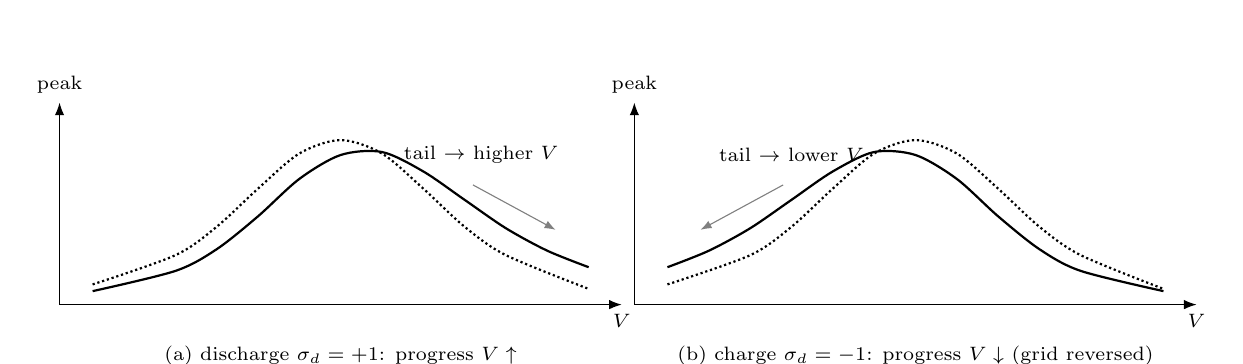
\begin{tikzpicture}[x=1.05cm,y=0.95cm]
% discharge panel (left)
\begin{scope}
\draw[-{Latex[length=1.6mm]}] (-3.4,0) -- (3.4,0) node[below,font=\scriptsize] {$V$};
\draw[-{Latex[length=1.6mm]}] (-3.4,0) -- (-3.4,2.7) node[above,font=\scriptsize] {peak};
% bell (equilibrium) dotted
\draw[densely dotted,thick] plot[smooth] coordinates {(-3,0.27) (-2,0.66) (-1.5,1.04) (-1,1.55) (-0.5,2.02) (0,2.2) (0.5,2.02) (1,1.55) (1.5,1.04) (2,0.66) (3,0.21)};
% discharge tail: shifted/broadened to higher V (right)
\draw[thick] plot[smooth] coordinates {(-3,0.18) (-2,0.45) (-1.5,0.74) (-1,1.18) (-0.5,1.68) (0,2.0) (0.5,2.04) (1,1.78) (1.5,1.4) (2,1.02) (2.5,0.72) (3,0.5)};
\draw[-{Latex[length=1.4mm]},gray] (1.6,1.6)--(2.6,1.0);
\node[font=\scriptsize] at (1.7,2.0) {tail $\to$ higher $V$};
\node[font=\scriptsize,below] at (0,-0.42) {(a) discharge $\sigma_d=+1$: progress $V\uparrow$};
\end{scope}
% charge panel (right)
\begin{scope}[xshift=7.3cm]
\draw[-{Latex[length=1.6mm]}] (-3.4,0) -- (3.4,0) node[below,font=\scriptsize] {$V$};
\draw[-{Latex[length=1.6mm]}] (-3.4,0) -- (-3.4,2.7) node[above,font=\scriptsize] {peak};
\draw[densely dotted,thick] plot[smooth] coordinates {(-3,0.27) (-2,0.66) (-1.5,1.04) (-1,1.55) (-0.5,2.02) (0,2.2) (0.5,2.02) (1,1.55) (1.5,1.04) (2,0.66) (3,0.21)};
% charge tail: mirror — broadened to lower V (left)
\draw[thick] plot[smooth] coordinates {(-3,0.5) (-2.5,0.72) (-2,1.02) (-1.5,1.4) (-1,1.78) (-0.5,2.04) (0,2.0) (0.5,1.68) (1,1.18) (1.5,0.74) (2,0.45) (3,0.18)};
\draw[-{Latex[length=1.4mm]},gray] (-1.6,1.6)--(-2.6,1.0);
\node[font=\scriptsize] at (-1.5,2.0) {tail $\to$ lower $V$};
\node[font=\scriptsize,below] at (0,-0.42) {(b) charge $\sigma_d=-1$: progress $V\downarrow$ (grid reversed)};
\end{scope}
\end{tikzpicture}
\caption{[Origin: v7-11 candidate] 인과 꼬리의 방향(신규). 점선 $=$ 평형 종($\xi_\eq(1-\xi_\eq)/w$, 방향 불변). 실선 $=$ peak\_shape with tail.
(a) 방전은 진행이 $V\!\uparrow$ 라 꼬리가 높은 $V$ 쪽으로 늘어진다(격자 그대로). (b) 충전은 진행이 $V\!\downarrow$ 라
격자를 뒤집어 필터($\xi[::-1]\cdots[::-1]$)해 꼬리가 낮은 $V$ 쪽으로 — 방전의 거울. 두 경우 모두 peak 는 양수.}
\label{fig:reversal}
\end{figure}

% ====================================================================
\section{합산과 역보간 (N9)}\label{sec:sum}
% ====================================================================
전이 루프가 각 전이의 peak\_shape 를 (식~\eqref{eq:branch} 의 두 분기로) 만들면, 코드는 용량 가중을 곱해 작업 격자 위
누적에 더하고, 모든 전이가 끝나면 내부 전위 격자로 역보간한다. 보존식 $Q_\cell q=Q_\bg+\sum_jQ_j\xi_j$ 가
$\sum_jQ_j\xi_j$ 꼴이라 관측 ICA 는 배경과 전이별 기여의 선형 합이다:

\begin{derivebox}
\textbf{합산 유도 사슬.} 출발점은 다시 보존식의 선형 분해다.
\begin{equation*}
Q_{\cell}q=Q_{\bg}(V_n)+\sum_{j=1}^{N_p}Q_j\xi_j.
\end{equation*}
궤적 미분과 연쇄율을 적용하면
\begin{equation*}
\frac{\dd Q}{\dd V_n}=C_{\bg}+\sum_j Q_j\frac{\dd\xi_j}{\dd V_n}.
\end{equation*}
각 전이의 $\dd\xi_j/\dd V_n$ 를 N6 의 평형 종 또는 N8 의 인과 기억 \code{peak\_shape} 로 대체하면, 코드에서는 먼저 작업 격자에
\begin{equation*}
\code{dqdv\_work}\leftarrow C_{\bg}(V_{\work})+\sum_j Q_j\code{peak\_shape}_j
\end{equation*}
를 만들고 마지막에 $V_n$ 으로 역보간한다. 따라서 합산은 별도 피팅 가정이 아니라 보존식 미분의 직접 결과다.
\end{derivebox}

\begin{equation}
\boxed{\;\frac{\dd Q}{\dd V}(V_n)\;=\;C_\bg\;+\;\sum_{j=1}^{N_p}Q_j\,
\big[\text{peak\_shape}_j\big]
\;=\;C_\bg+\sum_jQ_j\big[\text{평형 peak}-\text{지연 꼬리}\big]\;.}
\label{eq:sum}
\end{equation}
코드는 \code{dqdv\_work += tr['Q'] * peak\_shape} 로 누적하고(배경은 루프 전에 깔림), 마지막에
\code{np.interp(V\_n, V\_work, dqdv\_work)} 로 작업 격자에서 내부 전위 격자로 되돌린다(\code{dqdv\_out}).
스칼라 입력이면 첫 성분만 반환한다.

\subsection{staging 전이 초기값 — 피팅 출발점}
4건의 전이 초기값이 \code{GRAPHITE\_STAGING\_LIT} 에 박혀 있다(신뢰값 아닌 \emph{초기값} — 사용자 피팅이 override
전제). 표~\ref{tab:staging} 가 각 인자의 의미와 출발값이다 — 이 표가 있어 ``이 문건만으로 곡선 재현 코드를 짤 수 있다''.

\begin{table}[t]
\centering
\renewcommand{\arraystretch}{1.25}
\caption{전이 초기값 \code{GRAPHITE\_STAGING\_LIT}(4건) — 출발점, 피팅으로 override. $U$ 는 \code{'U'}
폴백이자 $(\Delta H_\rxn,\Delta S_\rxn)$ 정합 목표.}
\label{tab:staging}
\begin{tabular}{l c c c c c c c}
\toprule
stage & $U$ [V] & $\Delta H_\rxn$ & $\Delta S_\rxn$ & $Q$ & $\Omega$ & $\Delta H_a$ & $|\dd V/\dd q|_{q_a}$ \\
 &  & [J/mol] & [J/(mol\,K)] & [$Q_\cell$] & [J/mol] & [J/mol] & [V] \\
\midrule
$4\!\to\!3$   & 0.210 & $-11700$ & $+29.0$ & 0.10 & 6000  & 48000 & 0.30 \\
$3\!\to\!2\mathrm L$ & 0.140 & $-13500$ & $0.0$   & 0.12 & 8000  & 46000 & 0.30 \\
$2\mathrm L\!\to\!2$ & 0.120 & $-13100$ & $-5.0$  & 0.25 & 10000 & 44000 & 0.30 \\
$2\!\to\!1$   & 0.085 & $-13000$ & $-16.0$ & 0.50 & 13000 & 40000 & 0.30 \\
\bottomrule
\end{tabular}
\end{table}

각 전이는 폭 $w$ 폴백(0.020/0.016/0.014/0.012 V)과 $n=1$, $\Delta S_a=0$ 을 함께 갖는다. $\Delta H_\rxn/\Delta S_\rxn$
은 $U(298)$ 정합으로 정해졌고($U=(-\Delta H_\rxn+298.15\Delta S_\rxn)/F$ 가 표의 $U$ 와 일치), $\Delta H_a$ 는 저SOC$\to$
만충에서 감소하는 DFT 활성화 경향, $|\dd V/\dd q|_{q_a}$ 는 컷 OCV 기울기(피팅), $\Omega$ 는 정규용액 추정이다.

\subsection{전체 입력 인자와 기본값 — 피팅 준비}
사용자 목표는 이 모든 인자를 입력으로 노출해 측정 데이터에 Optuna 로 피팅하는 것이다. 곡선식의 모든 기호가 생성자 인자
또는 전이 dict 키이며, 내부 하드코딩 상수는 없다(전부 기본값$+$override). 표~\ref{tab:inputs} 가 전 조정 인자와
기본값이다 — 어느 것을 고정하고 어느 것을 피팅할지는 사용자가 데이터로 정한다(본 문건은 스코프를 정하지 않는다).

\begin{table}[t]
\centering\footnotesize
\renewcommand{\arraystretch}{1.18}
\caption{전체 입력 인자(코드 식별자)와 기본값. 전이 dict 키는 전이별, 생성자 인자는 모델 공통이며 일부는 전이 dict 로
per-transition override 된다($z_\mathrm{cut}$,$A_\mathrm{cap}$,\code{use\_w\_eff},\code{use\_dH\_eff}).}
\label{tab:inputs}
\begin{tabular}{l l l l}
\toprule
인자(코드) & 자리 & 기본값 & 곡선 내 역할(식) \\
\midrule
\multicolumn{4}{l}{\emph{— 전이 dict 키(전이별) —}}\\
\code{U} 또는 (\code{dH\_rxn},\code{dS\_rxn}) & 전이 & --- & 평형 중심 $U_j(T)$ (\eqref{eq:Uj}) \\
\code{w} 또는 \code{n} & 전이 & --- / $1$ & 폭 $w_j=n_jRT/F$ (\eqref{eq:wbase}) \\
\code{Q} & 전이 & --- & 용량 가중(면적) \\
\code{Omega},\code{gamma} & 전이 & $0$,\,$0$ & 상호작용$\cdot$분기(히스, \eqref{eq:dUhys}\eqref{eq:Ubranch}) \\
\code{h\_eta} & 전이 & $1.0$ & 부분 cycle 분기 인자 \\
\code{dH\_a},\code{dS\_a} & 전이 & --- / $0$ & 활성화(꼬리, \eqref{eq:Lqfull}) \\
\code{dVdq\_qa} & 전이 & $0$ & 컷 OCV 기울기 $L_q\!\to\!L_V$ (\eqref{eq:LV}) \\
\code{L\_V} & 전이 & --- & 직접 지연 길이(동역학 우회) \\
\code{z\_cut},\code{A\_cap\_RT} & 전이/공통 & $4.357$,\,$4.0$ & 컷 affinity (\eqref{eq:Acut}) \\
\code{use\_w\_eff},\code{use\_dH\_eff} & 전이/공통 & False,\,True & 옵션 토글(\eqref{eq:weff},\eqref{eq:dHeff}) \\
\multicolumn{4}{l}{\emph{— 생성자 인자(모델 공통) —}}\\
\code{x}/\code{chi},\,\code{chi\_split} & 공통 & $0.5$,\,\code{func\_chi\_d} & 전달 계수 $\chi_d$ (\eqref{eq:chid}) \\
\code{Rn} & 공통 & $0.0$ & 분극 저항 (\eqref{eq:vn}) \\
\code{Cbg} & 공통 & $0.0$ & 배경 $C_\bg$ (상수 또는 $V$ 함수) \\
\code{w\_eff\_floor\_frac} & 공통 & $0.05$ & $w^\eff$ 하한 분율 (\eqref{eq:weff}) \\
\code{grid\_pad\_lo/hi},\,\code{n\_work\_min} & 공통 & $0.15$,\,$2048$ & 작업 격자 (\eqref{eq:vwork}) \\
\code{min\_lag\_grid\_steps} & 공통 & $2.0$ & 꼬리/평형 전환 문턱 (\eqref{eq:branch}) \\
\code{v\_span\_floor} & 공통 & $10^{-6}$ & 격자 폭 하한(수치 안전) \\
\code{seed\_T/I/Q\_cell} & 공통 & $298.15$,\,$0.1$,\,$1.0$ & 진단용 seed $L_V$ 대표 조건 \\
\multicolumn{4}{l}{\emph{— 호출 인자(\code{curve}/\code{dqdv}) —}}\\
\code{V\_app},\code{T},\code{c\_rate}/\code{I\_abs},\code{Q\_cell},\code{direction} & 호출 & --- & 실험조건 (\eqref{eq:n0map}) \\
\bottomrule
\end{tabular}
\end{table}

표의 모든 행이 코드 입력이라 ``고정/피팅 스코프''는 자유롭게 잡을 수 있다 — 예컨대 $(\Delta H_\rxn,\Delta S_\rxn,Q,w)$ 를
풀고 $(\Omega,\Delta H_a,\code{dVdq\_qa})$ 는 좁은 상하한으로 두는 식이다. 리액션$\cdot$DFT 값은 신뢰 상한이 아니라
\emph{출발점}이므로 소폭 자유도를 권한다.

\begin{keybox}
\textbf{이 문건만으로 한 곡선 재현(6단계).}
(1) 표~\ref{tab:staging} 의 4 전이로 \code{transitions} 구성.
(2) 실험조건 $\sigma_d$, $|I|=\code{c\_rate}\cdot Q_\cell$, $T$, $R_n$ 설정 → 분극 $V_n$(\eqref{eq:n0map}\eqref{eq:vn}), 작업 격자 $V_\work$(\eqref{eq:vwork}).
(3) 전이마다 $U_j(T)$(\eqref{eq:Uj}) → 분기 중심 \code{center}(\eqref{eq:center}) → 폭 $w_j$(\eqref{eq:wbase}) → 평형 점유 $\xi_\eq$(\eqref{eq:xieq}).
(4) 지연 길이: $\mathcal A$(\eqref{eq:Acut}) → $\chi_d,\Delta H_a^\eff$(\eqref{eq:chid}\eqref{eq:dHeff}) → $L_q$(\eqref{eq:Lqfull}) → $L_V$(\eqref{eq:LV}), 전이당 상수.
(5) peak\_shape: $L_V<2\Delta_\mathrm{grid}$ 면 평형 종(\eqref{eq:eqpeak}), 아니면 인과 꼬리(\eqref{eq:peakshape}, 충전 격자 역전 \eqref{eq:reversal}).
(6) 용량 가중 합산 후 $V_n$ 으로 역보간(\eqref{eq:sum}). 색인은 표~\ref{tab:nodemap}.
\end{keybox}

\subsection{facade 와 전체 진행 한눈에}
상위 \code{curve} 가 실험조건을 받아 $\sigma_d=\code{\_direction\_to\_sigma}$, $|I|=\code{c\_rate}\cdot Q_\cell$
(또는 \code{I\_abs} 우선)로 환산해 \code{dqdv} 를 재사용한다(새 물리 없음). 기준선 \code{equilibrium} 은
$|I|\to0$ 한계로 식~\eqref{eq:eqpeak} 만 합산한 충방전 불변$\cdot$히스 미반영 곡선이다. 전체 진행은 표~\ref{tab:nodemap}
가 노드$\cdot$식$\cdot$코드 식별자로 닫는다.

\begin{table}[t]
\centering
\renewcommand{\arraystretch}{1.3}
\caption{노드 $\leftrightarrow$ 식 $\leftrightarrow$ 코드 식별자 매핑(전체 진행). 본 문건 절 순서 $=$ 이 노드 순서.}
\label{tab:nodemap}
\begin{tabular}{l l l l}
\toprule
노드 & 물리식 & 본 문건 식 & 코드 식별자 \\
\midrule
N0 & $\sigma_d,|I|=\code{c\_rate}\,Q_\cell$ & \eqref{eq:n0map} & \code{curve},\code{\_direction\_to\_sigma} \\
N1 & $V_n=V_\app-\sigma_d|I|R_n$ & \eqref{eq:vn} & \code{dqdv} L412 \\
N2 & $U_j(T)=(-\Delta H+T\Delta S)/F$ & \eqref{eq:Uj} & \code{func\_U\_j} \\
N3 & $\Delta U_j^\hys$, $U_j^{\,d}$ & \eqref{eq:dUhys},\eqref{eq:Ubranch} & \code{func\_dU\_hys},\code{func\_U\_branch} \\
N4 & $w_j=n_jRT/F$ ($w^\eff$) & \eqref{eq:wbase}(\eqref{eq:weff}) & \code{func\_w},\code{func\_w\_eff},\code{\_width} \\
N5 & $\xi_\eq=\mathrm{logistic}[\sigma_d(V-U^d)/w]$ & \eqref{eq:xieq} & \code{func\_ksi\_eq} \\
N6 & $Q_j\xi_\eq(1-\xi_\eq)/w$ & \eqref{eq:eqpeak} & \code{equilibrium}, 인라인 \\
N7 & $\mathcal A,\chi_d,\Delta H_a^\eff,L_q,L_V$ & \eqref{eq:Acut}--\eqref{eq:LV} & \code{\_resolve\_lag\_length},\code{func\_L\_q} \\
N8 & $(\xi_\eq-\xi_\mathrm{lag})/L_V$, 역전 & \eqref{eq:peakshape},\eqref{eq:reversal} & \code{\_causal\_lowpass} \\
N9 & $C_\bg+\sum_jQ_j[\cdot]$ & \eqref{eq:sum} & \code{dqdv\_work},\code{np.interp} \\
\bottomrule
\end{tabular}
\end{table}

% ====================================================================
\section{부호 사슬 전수 검산}\label{sec:signcheck}
% ====================================================================
브리프 §8 의 부호 체크리스트를 전건 확인한다 — 한 곳이라도 어긋나면 결함이다. 기준 명제 = \emph{방전 시
$V\!\uparrow\Rightarrow$ 탈리튬화$\uparrow$, 충전 $\dd Q/\dd V$ 는 방전의 거울(양수)}.

\begin{enumerate}[label=\textbf{S\arabic*.},leftmargin=2.6em,itemsep=2pt]
\item \textbf{$U_j(T)=(-\Delta H+T\Delta S)/F$, $\Delta G=-FU$.} 식~\eqref{eq:Uj}$\cdot$\eqref{eq:eqcond}. $\Delta H_\rxn<0$
(발열)이면 $-\Delta H_\rxn>0$ 이 중심을 올린다(흡열 아님). $\Delta G_j=-sFU_j$ 부호 일치. $\checkmark$
\item \textbf{$\xi_\eq=\mathrm{logistic}[\sigma_d(V-U)/w]$.} 식~\eqref{eq:xieq}. 방전 $\sigma_d=+1$ 에서
$V\!\uparrow\Rightarrow\xi_\eq\!\uparrow$. $\checkmark$
\item \textbf{$d\xi/dV=\sigma_d\,\xi(1-\xi)/w$, peak 양수.} 식~\eqref{eq:eqpeak}. peak 모양 $=|\dd\xi/\dd V|=
\xi(1-\xi)/w\ge0$, 방향 불변. $\checkmark$
\item \textbf{$\Delta U_\hys\ge0$, $\Omega\le2RT\to0$; 분기 중심 $\pm\tfrac12\sigma_d$.} 식~\eqref{eq:dUhys}$\cdot$
\eqref{eq:Ubranch}. 극대 $>$ 극소라 $\ge0$; $u_j\to0$ 에서 $0$; 방전 $+$/충전 $-$ 라 $U^{\dis}>U^{\chg}$. $\checkmark$
\item \textbf{$\chi_d$: 방전 $\chi$/충전 $1-\chi$; $\Delta H_a^\eff=\Delta H_a-\chi_d\Omega$.} 식~\eqref{eq:chid}$\cdot$
\eqref{eq:dHeff}. 합-1 거울 대칭. $\checkmark$
\item \textbf{$\partial\ln L_q/\partial V<0$ (물리적 동기).} 식~\eqref{eq:Lqfull}$\cdot$\eqref{eq:LV} 논의. $\mathcal A$ 가
컷 상수라 \emph{운영상 실현 미분은} $\partial\ln L_q/\partial V=0$(전이당 한 스칼라)이고, 부등식 $<0$ 은 컷 규칙의
\emph{동기}로만 성립한다 — 국소 구동력으로 두면 $V\!\uparrow\Rightarrow\mathcal A\!\uparrow\Rightarrow$ 유효 장벽
$\downarrow\Rightarrow L_q\downarrow$(꼬리 짧아짐). 자기모순 없음(동결과 부등식이 같은 단조성에서 일관). $\checkmark$
\item \textbf{꼬리: 충전 격자 역전($\xi[::-1]\cdots[::-1]$); 충전 $\dd Q/\dd V$ 방전 거울(양수).} 식~\eqref{eq:reversal}.
인과 방향 보존, peak\_shape $=(\xi_\eq-\xi_\mathrm{lag})/L_V>0$. $\checkmark$
\item \textbf{분극 $V_n=V_\app-\sigma_d|I|R_n$.} 식~\eqref{eq:vn}. 방전 시 측정 $>$ 내부 보정. $\checkmark$
\end{enumerate}
전건이 기준 명제와 정합한다 — 부호 결함 $0$.

\begin{verifybox}
\textbf{부호 회귀 self-test (재현 가능 수치 고정).} 위 정성 검산을 falsifiable 수치에 못박아 회귀를 막는다 — 아래
네 항은 코드 \code{\_\_main\_\_} 의 self-test 와 같은 양을 손으로 재산출한 것이며($T=298.15$ K), 한 줄이라도 어긋나면
부호 사슬이 깨진 것이다.
\begin{enumerate}[label=\textbf{R\arabic*.},leftmargin=2.6em,itemsep=1pt]
\item \textbf{히스 분기 방향.} $\Omega=12000$ J/mol, $\gamma=1$ 에서 식~\eqref{eq:dUhys} 는
$\Delta U^\hys=\frac{2}{F}[\Omega u-2RT\,\mathrm{artanh}\,u]=86.7$ mV($u=\sqrt{1-2RT/\Omega}=0.766$). 분기 중심
식~\eqref{eq:Ubranch} 가 방전 $+\tfrac12\Delta U^\hys$/충전 $-\tfrac12\Delta U^\hys$ 라, peak 갈림
$V_\dis-V_\chg=+\gamma\,\Delta U^\hys=+86.7$ mV $>0$(방전 peak 가 높은 전위 — 기준 명제 일치).
\item \textbf{히스 문턱.} $\Omega=2RT=4958$ J/mol 에서 $u=0$, 식~\eqref{eq:dUhys} $\Rightarrow\Delta U^\hys=0.0$ mV —
$\Omega\le2RT$ 분기가 정확히 $0$ 으로 연속(상분리 미만 = 갈림 없음).
\item \textbf{$|I|\!\to\!0$ 환원·방향 불변.} $\gamma=0$, $|I|=10^{-6}$ 에서 식~\eqref{eq:LV} 의 $L_V\propto|I|\to0$ 이라
식~\eqref{eq:branch} 가 평형 종으로 떨어지고, 식~\eqref{eq:eqpeak} 의 peak $=\xi_\eq(1-\xi_\eq)/w$ 는 $\sigma_d$ 불변 —
방전$\cdot$충전 곡선 차 $\to0$(부호 $S3$ 의 양수$\cdot$방향 불변 수치 확인).
\item \textbf{$L_q$ 동결 vs 부등식.} $\mathcal A=\min(z_\mathrm{cut}n_jRT,A_\mathrm{cap}RT)$ 가 전이당 상수라
$\partial\ln L_q/\partial V=0$(실현 미분)이고, 부등식 $\partial\ln L_q/\partial V<0$ 은 컷 규칙 동기로만 성립한다($S6$ 의
정정과 일관) — 두 진술이 한 단조성을 공유하므로 자기모순 $0$.
\end{enumerate}
네 회귀 항이 모두 통과한다 — 부호 사슬 self-test PASS.
\end{verifybox}

% ====================================================================
\begin{thebibliography}{9}
\bibitem{dahn1991} J. R. Dahn, ``Phase diagram of Li$_x$C$_6$,'' \emph{Phys. Rev. B} \textbf{44}, 9170 (1991). DOI: 10.1103/PhysRevB.44.9170.
\bibitem{ohzuku1993} T. Ohzuku, Y. Iwakoshi, K. Sawai, ``Formation of Lithium-Graphite Intercalation Compounds in Nonaqueous Electrolytes,'' \emph{J. Electrochem. Soc.} \textbf{140}, 2490 (1993). DOI: 10.1149/1.2220849.
\bibitem{bazant2013} M. Z. Bazant, ``Theory of Chemical Kinetics and Charge Transfer based on Nonequilibrium Thermodynamics,'' \emph{Acc. Chem. Res.} \textbf{46}, 1144 (2013). DOI: 10.1021/ar300145c.
\bibitem{eyring1935} H. Eyring, ``The Activated Complex in Chemical Reactions,'' \emph{J. Chem. Phys.} \textbf{3}, 107 (1935). DOI: 10.1063/1.1749604.
\bibitem{dreyer2010} W. Dreyer \emph{et al.}, ``The thermodynamic origin of hysteresis in insertion batteries,'' \emph{Nature Materials} \textbf{9}, 448 (2010). DOI: 10.1038/nmat2730.
\bibitem{bloom2005} I. Bloom \emph{et al.}, ``Differential voltage analyses of high-power, lithium-ion cells,'' \emph{J. Power Sources} \textbf{139}, 295 (2005). DOI: 10.1016/j.jpowsour.2004.07.021.
\bibitem{dubarry2012} M. Dubarry, C. Truchot, B. Y. Liaw, ``Synthesize battery degradation modes via a diagnostic and prognostic model,'' \emph{J. Power Sources} \textbf{219}, 204 (2012). DOI: 10.1016/j.jpowsour.2012.07.016.
\end{thebibliography}

\end{document}
